%TODO
% 4 improve technique, eval. 
% 5 related work, proofread...

\documentclass[conference]{IEEEtran}

\usepackage{graphicx}
\usepackage[usenames,dvipsnames]{color}
\usepackage{algpseudocode}
\usepackage{ amssymb}
\usepackage{url}

\usepackage{amsthm, amsmath, amssymb}
%\usepackage{amsthm}
% conflict with the following commands
%\newdef{definition}{Definition}
\newtheorem{definition}{Definition}
\newtheorem{mydiscussion}{Discussion}
\newtheorem{myproof}{Proof Sketch}
\newtheorem{mytheorem}{Theorem}
\newtheorem{myproperty}{Property}
\newtheorem{myrule}{Rule}

\newcommand{\sysname}{{\sc Recipe}}
\newcommand{\tool}{{\sc Recipe}}
\newcommand{\lsyn}{\lbrack\!\lbrack}
\newcommand{\rsyn}{\rbrack\!\rbrack}


\setcounter{secnumdepth}{3}


\ifCLASSINFOpdf
  % \usepackage[pdftex]{graphicx}
  % declare the path(s) where your graphic files are
  % \graphicspath{{../pdf/}{../jpeg/}}
  % and their extensions so you won't have to specify these with
  % every instance of \includegraphics
  % \DeclareGraphicsExtensions{.pdf,.jpeg,.png}
\else
  % or other class option (dvipsone, dvipdf, if not using dvips). graphicx
  % will default to the driver specified in the system graphics.cfg if no
  % driver is specified.
  % \usepackage[dvips]{graphicx}
  % declare the path(s) where your graphic files are
  % \graphicspath{{../eps/}}
  % and their extensions so you won't have to specify these with
  % every instance of \includegraphics
  % \DeclareGraphicsExtensions{.eps}
\fi


\hyphenation{op-tical net-works semi-conduc-tor}

\usepackage{listings}

\lstset{
	numbers=left,
	numberstyle=\tiny,
	language={Java},
	mathescape=true,
	flexiblecolumns=true,
	morekeywords={def,Int,call,method,var,assert,share,unshare,acquire,release,fork,join,free,invariant,requires,ensures,acc,rd,old},
	basicstyle=\sffamily\small,
	moredelim=[is][\itshape]{@}{@},
	stepnumber=1,
	numbersep=2pt} 

\begin{document}
%
% paper title
% can use linebreaks \\ within to get better formatting as desired
\title{\tool: Relaxed Sound Predictive Analysis}


% author names and affiliations
% use a multiple column layout for up to three different
% affiliations
%\author{\IEEEauthorblockN{Michael Shell}
%\IEEEauthorblockA{School of Electrical and\\Computer Engineering\\
%Georgia Institute of Technology\\
%Atlanta, Georgia 30332--0250\\
%Email: http://www.michaelshell.org/contact.html}
%\and
%\IEEEauthorblockN{Homer Simpson}
%\IEEEauthorblockA{Twentieth Century Fox\\
%Springfield, USA\\
%Email: homer@thesimpsons.com}
%\and
%\IEEEauthorblockN{James Kirk\\ and Montgomery Scott}
%\IEEEauthorblockA{Starfleet Academy\\
%San Francisco, California 96678-2391\\
%Telephone: (800) 555--1212\\
%Fax: (888) 555--1212}}

% conference papers do not typically use \thanks and this command
% is locked out in conference mode. If really needed, such as for
% the acknowledgment of grants, issue a \IEEEoverridecommandlockouts
% after \documentclass

% for over three affiliations, or if they all won't fit within the width
% of the page, use this alternative format:
%
%\author{\IEEEauthorblockN{Michael Shell\IEEEauthorrefmark{1},
%Homer Simpson\IEEEauthorrefmark{2},
%James Kirk\IEEEauthorrefmark{3},
%Montgomery Scott\IEEEauthorrefmark{3} and
%Eldon Tyrell\IEEEauthorrefmark{4}}
%\IEEEauthorblockA{\IEEEauthorrefmark{1}School of Electrical and Computer Engineering\\
%Georgia Institute of Technology,
%Atlanta, Georgia 30332--0250\\ Email: see http://www.michaelshell.org/contact.html}
%\IEEEauthorblockA{\IEEEauthorrefmark{2}Twentieth Century Fox, Springfield, USA\\
%Email: homer@thesimpsons.com}
%\IEEEauthorblockA{\IEEEauthorrefmark{3}Starfleet Academy, San Francisco, California 96678-2391\\
%Telephone: (800) 555--1212, Fax: (888) 555--1212}
%\IEEEauthorblockA{\IEEEauthorrefmark{4}Tyrell Inc., 123 Replicant Street, Los Angeles, California 90210--4321}}




% use for special paper notices
%\IEEEspecialpapernotice{(Invited Paper)}




% make the title area
\maketitle

\begin{abstract}
Predictive analysis has recently emerged as a promising paradigm for sound detection of multithreading bugs (i.e., without false alarms). The idea is to start from an instrumented execution trace, and transform it based on the concrete information it provides (e.g., concrete values and memory accesses) while preserving feasibility (e.g., by reodering trace events iff flow dependencies are preserved), such that bugs are exposed.

Predictive analysis has been applied successfully to the problem of data-race detection, though state-of-the-art techniques are restrictive in the transformations they allow so as to guarantee feasibility and consequently also soundness. In particular, existing techniques (i) do not permit flow dependencies to be violated (except in very specific cases), and (ii) are unable to analyze execution paths beyond that of the input trace.

In this paper, we present \sysname, a predictive race detector that is able to relax both of these restrictions while guaranteeing soundness, as we prove formally. Thanks to its ability to explore event orderings that violate flow dependencies as well as unexecuted branches, \sysname\ is able to detect x$2.5$ more data races on a representative set of large-scale benchmarks compared to the state of the art in predictive race detection.
\end{abstract}

% IEEEtran.cls defaults to using nonbold math in the Abstract.
% This preserves the distinction between vectors and scalars. However,
% if the conference you are submitting to favors bold math in the abstract,
% then you can use LaTeX's standard command \boldmath at the very start
% of the abstract to achieve this. Many IEEE journals/conferences frown on
% math in the abstract anyway.

% no keywords




% For peer review papers, you can put extra information on the cover
% page as needed:
% \ifCLASSOPTIONpeerreview
% \begin{center} \bfseries EDICS Category: 3-BBND \end{center}
% \fi
%
% For peerreview papers, this IEEEtran command inserts a page break and
% creates the second title. It will be ignored for other modes.
\IEEEpeerreviewmaketitle



%Limitations of static analysis: scalability when it is path sensitive, difficulty in modeling heap, cannot reason about concrete values, have to use
%abstraction, so that may not be sound, dynamic analysis is precise, easily scale to long and complex runs, but it only reasons about problems that
%did occur. 

%Predictive analysis is so good

%But it restricts too much, only relax schedule space and a little bit of the dependence space.

%We observe many dynamic aspects can be relaxed without affecting soundness.  as a result, instead of reasoning one
%execution, we can reason the neighborhood of the execution, in order words, we leverage dynamic analysis to provide
%the information that is difficult to analyze statically such as aliasing and a long execution path that covers the
%intended workflow, then we relax the predictive analysis to analyze neighborhood.  


\section{Introduction}\label{Se:introduction}
Program analyses can be largely classified to static and dynamic analyses. Static analyses abstract programs statically.
They are usually complete and do not require concrete program inputs to drive the analyses. However, they have difficulty in
scaling to large and complex programs when the analyses are path-sensitive, due to the sheer number of paths and the 
complexity of the paths. Path-insensitive analyses often do not have sufficient precision on the other hand. 
Static analyses also have difficulty in modeling complex aliasing behavior. In contrast, dynamic analysese focus 
on analyzing a few executions, usually just one. They are sound and easily scale to long and complex executions. But they 
can only reason about properties that manifest themselves in the execution(s). 

Recently, a novel kind of analysis called predictive analysis~\cite{...} was proposed. It has the capabilities of 
achieving soundness as dynamic analyses and reasoning about properties that did not occur during execution 
just like in static analysis. The basic idea is to leverage dynamic analysis to provide the information that 
is difficult to acquire through static analysis, such as a complex execution path that covers important functionalities 
and aliasing information. Note that during execution, we know precisely which write access reaches any given read 
access. While such information is encoded in a trace, predictive analysis reaons about mutation of the trace to 
expose problems or study properties that may not manifest during execution. It was used in sound data race detection. 
In particular, it collects a trace of threaded execution that contains rich runtime information such as concrete values, 
execution path, and memory accsses. It then leverages constraint solving to reason about if races can occur with
a different thread schedule, {\em while enforcing the critical runtime information (e.g. values, thread
local paths, and memory accesses) remains the same during schedule pertubation}. The rationale is that 
it becomes as difficult as static analysis if we allow these critical runtime information change. 
Preditive analysis has been shown to be very effective. It can detect real data races from complex programs.
And more importantly, it guarantees the results are sound (i.e. no false positives).

Despite its effectiveness, we observe that existing predictive analyes are too restrictive. They 
require too much runtime information to remain unchanged during analysis such that coverage is unnecessarily
limited. 


\begin{figure}
\centering
\begin{tabular}{ll}
\multicolumn{2}{c}{{\tt x = 0; y = 0;}} \\  % z = 3;
%\multicolumn{2}{c}{{\color{red} {\tt z = 2;}}} \\
\hline
\multicolumn{1}{c}{$T_1$} & \multicolumn{1}{c}{$T_2$} \\
\hline
{\tt 1: y = 3;} & \\
{\tt 2: x = 1;} & \\
{\tt 3: y = 5;} & \\
& {\tt 4: if (y > 2)} \\
& {\tt 5:~~z=1/x;} \\	
& {\color{red} {\tt 6: else}} \\
& {\color{red} {\tt 7:~~w=2/x;}}
\end{tabular}
\caption{Example illustrating ordering constraints beyond synchronization primitives}
\label{fig:running}
\end{figure}

Consider the example in Figure \ref{fig:running}, which shows an execution trace of two threads. The statements in red 
denote an unexplored branch outside the trace. Existing predictive analyses are unable to detect the race between 
lines {\tt 2} and {\tt 5} because they require that during trace permutations (by different schedules), a variable must not have
a different value in a permuted trace\footnote{They allow the variable involved in a race to have different values.}.
As such, they cannot execute line {\tt 4} before line {\tt 3}, which is needed to expose the race between lines {\tt 2}
and {\tt 5}. 
%the dependence between lines {\tt 3} and {\tt 4}, which is a barrier to the needed reorderings. 
A second race between lines {\tt 2} and {\tt 7} is also missed as the mutated trace must have the same thread local
path as the original trace. 

However, we observe that such restrictions are unnecessary. For example, we can allow line {\tt 4} to receive its
value from line {\tt 1} as it has the same effect on thread local execution (i.e. the same branch is taken). 
However, the relaxation would allow us to execute lines {\tt 4} and {\tt 5} before line {\tt 2}, exposing 
the first missing race. We can also allow the trace to take the else branch such that the second race is also exposed. 
Note that even though the else branch was not executed originally, its effect can be precisely modeled as the value 
of $x$ is known from the original trace. As such, we can still perform sound analysis.

%that is missed, as it involves the statements in red, is between lines {\tt 2} and {\tt 7}.
Therefore in this paper, we propose \sysname, a relaxed predictive analysis. We identify the critical runtime
informantion that needs to be preserved during trace perturbation and relax the remaining information. 
In particular, we preserve all the addresses de-referenced (e.g. heap and array accesses) in the original execution,
and some of the branch outcomes such that part of the thread local paths stay intact. The criterion is that
we forbid \sysname to explore an unexecuted branch if the effect of the branch cannot be precisely modeled
(e.g. an array element is read while it was not defined in the original trace). The essence of our technique 
is to {\em explore the neighborhood of the original execution as much as possible}. Due to the substantially
enlarged search space, our results show that a race detector based on our relaxed predictive analysis 
can detect XXX times more races than existing predictive analysis, while guaranteeing soundness. 

Our contrituions are summarized as follows.
\begin{itemize}
\item We propose to relax existing preditive analysis and identify a bound of relaxation (i.e. what can
be relaxed).
\item We develop a constraint encoding scheme that uniformally encodes the strict information (i.e. the
part must be preserved) and the relaxed information. 
\item We develop a propotype \sysname. Our results show XXX.
\end{itemize}









\section{Technical Overview}\label{sec:overview}

In this section, we walk the reader through a detailed technical description of our approach based on the example in Figure \ref{fig:running}. 
%
As input, we assume (i) a program $P$ as well as (ii) a trace of $P$ recorded during a dynamic execution.

% in Static Single Assignment (SSA) form, such that every variable is defined exactly once.


\subsection{Preliminaries}
To facilitate our presentation, we first introduce some terminologies used throughout this paper. Intuitively, a trace is a sequence of events recorded during the observation run.




{\bf Event\ } An event, $e=<t, id, inst>$, is a concrete representation of the runtime execution of a static instruction $inst$.


\begin{itemize}
\item $t$ refers to the thread that issues the event $e$, denoted as $t^e$.
\item  $id$ refers to the id associated with each event. The key property of  $id$ is {\em uniqueness}, i.e., any two events in the trace own different ids.  Unless otherwise specified, we use  the index of an event in the trace as its id, which satisfies the above property. Throughout this paper,  we denote an event as $e_{id}$ with the id as the subscript. %We may use the terms $e_{id}$ and $id$ interchangeably given their one-to-one correspondence, e.g., $t^{e_3}$ and $t^3$. 
\item $inst$ is the static instruction. The instructions are three-address instructions involving at most three operands, which modern compilers commonly support.  Specifically, we are interested in the types of instructions listed in Table~\ref{Ta:syntax}. When the variable does not appear on the left hand of an equation, such as $y$ in $x.f=y$, it may refer to a variable, a constant or event object creation expression $new (...)$.  The $bop$ stands for the binary operator, which may refer to $+, -, *, /, \%, \wedge, \vee$ in the assignment, or refer to $<, >, =, \wedge, \vee$ in the branch. The target of the branch event is not important in our scope, therefore, we may abbreviate the branch instruction as the boolean expression afterwards. The listed instructions suffice to represent all trace events of interest. This is because a concrete finite execution trace can be reduced to a straight-line loop-free call-free path program  (argument passing of the method call is modeled as assignments and the virtual call resolution is modeled as branches). This standard form of simplification preserves all the data-race-related information contained in the original trace. 
\end{itemize}



\begin{table}
	\begin{center}
		\begin{tabular}{rcl}
			\multicolumn{1}{l}{{\tt s} $::=$} & & \\
			{\tt y = x.f} & $|$ & {\bf (heapr)} \\ 
			{\tt x.f = y}  & $|$ & {\bf (heapw)} \\ %\ $|$\ {\tt x.f = $c$}\
			{\tt z = x $bop$ y}\  & $|$ & {\bf (assign)} \\ %$|$\ {\tt z = $c$} $|$ {\tt z = new()}
			{\tt if (x $bop$  y) goto ...} & $|$ &  {\bf (branch)} \\
			{\tt lock(l)}\ $|$\ {\tt unlock(l)}  & $|$& {\bf (sync)} \\
			{\tt fork(t)}\ $|$\ {\tt join(t)}$|$ {\tt begin(t)}\ $|$\ {\tt end(t)} &  & {\bf (thread)}
		\end{tabular}
	\end{center}
	\caption{\label{Ta:syntax}Instruction Types}
\end{table}


{\bf Trace \ } A trace $\tau$ is a sequence of events. It can also be represented more comprehensively as,  $\tau=<\Gamma , \{\tau_{t_1}, \tau_{t_2}, \dots \tau_{t_n} \}, O, \theta>$.
\begin{itemize}
\item  $\Gamma$ refers to the set of threads involved in the trace, which include $t_1$, $t_2$, \dots, $t_n$.
\item   $\{\tau_{t_1}, \tau_{t_2}, \dots \tau_{t_n} \}$ denotes the event sequences produced by each thread.  
\item  $O$ is a function that assigns  to every event an integer value that denotes its scheduling order. For example, $e_i$ is scheduled earlier than $e_j$ if $O(e_i)<O(e_j)$.
\item  $\theta$ is a function that maps every variable to a value. For example, given an event $e$ executing the instruction $x=y+z$, the mapping recorded in the trace may be $\theta(x)=3$,  $\theta(y)=2$,  $\theta(z)=1$.  If the variable $x$ is defined in two events, the mapping for $x$ becomes ambiguous. To avoid the ambiguity, we conduct a pre-processing  (Section~\ref{sec:relax1}) that produces the SSA form of the trace, in which each variable is defined exactly once. 
\end{itemize}

%\item $map$ is a mapping from live expressions at the current event to their value (and thus a partial mapping from expressions to values). Live expressions include program variables, object fields, boolean expressions, etc. We use the notation $\lsyn exp \rsyn^e$ to retrieve the value associated with expression $exp$ at $e$.
%Specially,  we also store the heap location value  $\lsyn \overline{x.f} \rsyn^e$ for a field $x.f$. Note the difference between $\lsyn \overline{x.f} \rsyn^e$ and $\lsyn x.f \rsyn^e$, which represent the location and the value stored in it respectively. The location value $\lsyn \overline{x.f} \rsyn^e$ is computed as a pair $(\lsyn x \rsyn^e, f)$.


%We introduce the projection operation ``$\downarrow$'' to facilitate the reasoning of the trace:
%$\tau\downarrow_{t}$ contains only the (ordered) events from the thread $t$; $\tau\downarrow_{\ell}$ contains the events involving the location $\ell$; $\tau\downarrow_{\leq id}$ denotes the prefix of $e_{id}$, i.e., the events preceding the event $e_{id}$; $\tau\downarrow_{\geq id}$ denotes the events after $e_{id}$; $\tau\downarrow_{>=id1\wedge <=id2}$ denotes the events between $e_{id1}$ and $e_{id2}$.

%\begin{itemize}
%\item projection operation  : 
%%\item sets: $\mathcal{T}$ denotes the set of threads involved;  $\mathcal{L}$ denotes the set of memory locations involved; 
%%$\mathcal{SV}$ denotes the set of shared variables, which reference the shared locations, the shared location $l$ can be judged by counting the number of threads in $\tau\downarrow_{\ell}$;  $\mathcal{E}$ denotes the set of events involved.
%\end{itemize}






%We make use of the following helper functions:
%\begin{itemize}
%	\item ${\sf proj}\ t\ i$ projects trace $t$ onto all transitions involving thread $i$.
%	\item $t[k]$ obtains the $k$th transition within trace $t$.
%	\item ${\sf index}\ t\ \tau$ retrieves the index, or offset, of transition $\tau$ within trace $t$. When simply writing
%	${\sf index}\ \tau$ (while omitting the trace parameter) we refer to the index of $\tau$ within the original trace. 
%	\item ${\sf pre}\ t\ \tau$ is the prefix of trace $t$ preceding transition $\tau$. For the suffix beyond $\tau$, we 
%	use ${\sf post}\ t\ \tau$. Finally, ${\sf bet}\ t\ \tau_1\ \tau_2$ returns the transitions delimited by $\tau_1$ and $\tau_2$.
%\end{itemize}

%Throughout this paper, we assume a standard operational semantics, which defines (i) a mapping ${\sf thr}$ between
%execution threads, each having a unique identifier $i \in \mathbb{N}$, and their respective code, as well as (ii) per-thread stack and shared heap memory. 

%The code executed by a given thread follows the syntax in Table \ref{Ta:syntax}. The text of a program is a sequence of zero or more method declarations, as given in the definition of symbol {\tt p}. Methods accept zero or more arguments $\overline{{\tt x}}$, have a body ${\tt s}$, and may have a return value (which we leave implicit). For simplicity, we avoid from static typing as well as virtual methods. The body of a method consists of the core grammar for symbol {\tt s}. We avoid from specifying syntax checking rules, as the grammar is fully standard.

%For simplicity, we assume that in the starting state each thread points to a parameter-free method. In this way, we can simply assume an empty starting state (i.e., an empty heap), and eliminate complexities such as user-provided inputs and initialization of arguments with default values. These extensions are of course possible, and in practice we handle these cases, but reflecting them in the formalism would result in needless complications.

%As is standard, we assume an interleaved semantics of concurrency. A \emph{transition}, or \emph{event}, is of the form
%$\sigma \stackrel{i / {\tt s}}{\longrightarrow} \sigma'$, denoting that thread $i$ took an evaluation step
%in prestate $\sigma$, wherein atomic
%statement {\tt s} was executed, which resulted in poststate $\sigma'$. We refer to a sequence of transitions from
%the starting state to either an exceptional state (e.g., due to null dereference) or a state where all the threads have 
%reduced their respective code to $\epsilon$ as a \emph{trace}.


%TODO this section is inconsistent with others. change it!
\subsection{Constraint System}
The predictive analysis takes the program and a trace as the input.  Suppose it starts with the following trace of the program in  Figure \ref{fig:running}:  $e_1 e_2 e_3 e_4 e_5$, where the line number is used as the event id (subscript). A potential race is between the pair, $(e_2, e_5)$, as they access the shared variable $x$ from different threads and one is a write. 

Given the trace, $\tau=<\Gamma , \{\tau_{t_1}, \tau_{t_2}, \dots \tau_{t_n} \}, O, \theta>$, the predictive analysis computes a new trace,  $\tau'=<\Gamma , \{\tau_{t_1}, \tau_{t_2}, \dots \tau_{t_n} \}, O', \theta'>$. $\tau'$ preserves the same event sequence for each thread, i.e., $T_1$ still executes $e_1 e_2 e_3$ and $T_2$ still executes $e_4 e_5$, but it reschedules the events from different threads so that the potential race pair runs concurrently, i.e., $e_2$ and $e_5$ run concurrently. When the schedule changes, the variables may get different values. Therefore, we need to compute both the new schedule $O'$ and the new value mapping $\theta'$, in order to witness a race. To guarantee that $\tau'$ is a feasible trace of the program $P$, the computation needs to respect a set of constraints, which include the value constraints, control flow constraints and synchronization constraints~\footnote{We omit the synchronization constraints in this paper, which are already well explained in existing techniques~\cite{yannis, pecan}.}. We explain them briefly in the following. The full details are explained in Section~\ref{sec:relax1} and the feasibility guarantee is explained in Section~\ref{sec:guarantee}.




%The local accesses are not used in this example and therefore omitted.






%We begin with an explanation of the encoding process. The resulting formula is provided in Figure \ref{fig:encoding}. We describe the conjuncts comprising the formula one by one.

%\begin{figure*}
%	\begin{center}
%$$
%	\begin{array}{rcl}
%	& \left( O_1 < O_2 < O_3 \wedge O_4 < O_5 \wedge O_4 < O_7 \right) & \textbf{(program order)} \\
%\bigwedge & \left( W_{\tt x}^0 = 0 \wedge W_{\tt y}^0 = 0 \wedge W_{\tt z}^0 = 3 \wedge W_{\tt y}^1 = 3 \wedge 
%	W_{\tt x}^2 = 1 \wedge W_{\tt y}^3 = 5 \right) & \textbf{(variable definitions)} \\
%\bigwedge & \left(		(R_{\tt y}^4=W_{\tt y}^0 \wedge O_4 < O_1) \vee	
%(R_{\tt y}^4=W_{\tt y}^1 \wedge O_1 < O_4 < O_3) \vee
%(R_{\tt y}^4=W_{\tt y}^3 \wedge O_3 < O_4)
%		\right) & \textbf{(thread interference)} \\
%\bigwedge & R_{\tt y}^4 > 2 \equiv {\bf true} & \textbf{(path conditions)} \\
%\bigwedge & t^2 \neq t^5 \wedge (2\ writes\ {\tt x} \vee 5\ writes\ {\tt x}) \wedge O_2 = O_5 & \textbf{(race condition)}
%	\end{array} 
%$$
%\end{center}
%\caption{\label{fig:encoding}\tool\ encoding of the trace in Figure \ref{fig:running} as a constraint system}
%\end{figure*}


We first preprocess the trace as follows. We introduce symbols to replace the shared accesses in the instructions, e.g., We use $W^{id}_{x}$/$R^{id}_{x}$ to replace the write/read of the shared variable $x$ by the event $e_{id}$. %The rationale is explained in Section~\ref{sec:relax1}.

{\bf Race Condition\ } The potential race pair involves two accesses of the same shared location from different threads, where at least one access is a write. Given any potential race pair, e.g., ($e_2$, $e_5$), it is a real race if and only if the two accesses can occur at the same time (race condition), which is captured by the race condition constraint
$$
	O'(e_2) = O'(e_5)
$$.
The race condition constraint--- together with the other constraints --- guarantees the feasibility of the predicted race if a solution is found for the overall constraint system.

{\bf Intra-thread Constraints\ } The predictive analysis needs to preserve the same event sequence for each thread, which further requires 

\begin{itemize}
\item {\bf Control Flow Constraints\ } Each thread takes the same control flows (or branch decisions) to reproduce the events.
 For the running example (ignoring the statements in red), this yields:
$$
	\theta'(R_{\tt y}^4) > 2 \equiv {\bf true}
$$
That is, in the predicted trace $\tau'$, the value of variable {\tt y} read at $e_4$ should be greater than $2$. 


\item {\bf Intra-thread Order Constraints\ } The events should follow the same thread-local order as in the original trace. This constraint is imposed by the fact that the two runs share the same instruction sequence and take the same control flows. 
We yield the following formula:
$$
	O'(e_1) < O'(e_2) < O'(e_3) \wedge O'(e_4) < O'(e_5)
$$
That is, in the predicted trace $\tau'$, the three events from $T_1$ are ordered in the same way as in $\tau$, and similarly, the branch event $e_4$ in $T_2$ still executes before the event $e_5$ inside the branch body.

\item {\bf Intra-thread Value Constraints\ } The events should respect the value constraints imposed by each instruction.
 For our running example, we obtain:
$$
\begin{array}{l}
	\theta'(W_{\tt x}^0) = 0 \wedge \theta'(W_{\tt y}^0) = 0 \wedge \theta'(W_{\tt y}^1) = 3 \\ 
	\wedge	\theta'(W_{\tt x}^2) = 1 \wedge \theta'(W_{\tt y}^3) = 5
	\end{array}
$$
As an example, $\theta'(W_{\tt y}^3)= 5$ denotes that the predicted run still assigns the value 5 to the variable {\tt y}  at event $e_3$.
\end{itemize}

%The next set of constraints, denoted ${\tt w}^i=k$ for local variables and $W_{\tt w}^i=k$ for shared variables, capture variable definitions: Variable {\tt w} is assigned value $k$ at statement $i$.


%Indeed, this constraint is satisfied by the assignments to {\tt y} both at line {\tt 1} and at line {\tt 3}.


{\bf Inter-thread Value Constraints\ } The inter-thread value constraints capture what writes the read events read from and under what scheduling condition the value flow occurs.  The resulting formula for our example is
$$
\begin{array}{lcl}
	& & (\theta'(R_{\tt y}^4)=\theta'(W_{\tt y}^0) \wedge O'(e_4) < O'(e_1) ) \\
& \bigvee &
	(\theta'(R_{\tt y}^4)=\theta'(W_{\tt y}^1) \wedge O'(e_1) < O'(e_4) < O'(e_3)) \\
& \bigvee &
	(\theta'(R_{\tt y}^4)=\theta'(W_{\tt y}^3) \wedge O'(e_3) < O'(e_4))
\end{array}
$$    
Notice, importantly, that the formula associates the value constraints with the scheduling order constraints. 
 As an example, 
$\theta'(R_{\tt y}^4)=\theta'(W_{\tt y}^1) \wedge O'(e_1) < O'(e_4) < O'(e_3)$ means that, in the predicted run, the read $e_4$ reads from the write $e_1$, under the condition that $e_4$ happens after $e_1$ and no other  writes (such as $e_3$) interleave them.



{\bf Unexplored Branches\ } Beyond the encoding steps so far, which focus on the given trace, we can often encode constraints along unexplored branches. In our running example, this is essential to discover the race between lines {\tt 2} and {\tt 7}. We conduct the symbolic execution to exercise the unexplored branches, which returns a set of traces representing possible executions of the unexplored branch. Each trace is combined with the original trace to find races involving the accesses in the unexplored path. For the racy events, $e_2$ and $e_7$, we first specify the race condition constraint  $O'(e_2)=O'(e_7)$. In addition, we negate the path condition, thereby obtaining $\theta'(R_{\tt y}^4) > 2 \equiv {\bf false}$ in place of $\theta'(R_{\tt y}^4) > 2 \equiv {\bf true}$. We also model the other necessary constraints such as the intra-thread order constraint $O'(e_4) < O'(e_7)$, similar to the above analysis.

{\bf Constraint Solving\ } The formuals from the different encoding steps are conjoined and sent to the off-the-shelf solver such as {\sf z3}.  The race under analysis is real if the solver returns a solution, which includes the scheduling order and the values for the variables. 

{\bf Highlights \ } In this example, our analysis finds two more pairs of races than existing analyses~\cite{yannis, jeff}, which include $(e_2, e_5)$ and $(e_2, e_7)$.
The key insight for finding the first race is, we do not require $e_4$ to read from $e_3$ to retain the original value, as what existing approaches do, rather, we allow $e_4$ to read from $e_1$ while still preserving the feasibility of the branch. This relaxation allows the events after $e_4$ to run concurrently with the events before $e_3$, leading to the detection of the first race.  The key insight for finding the second race is, we explore the unexplored branches and ask the solver to compute a feasible schedule that exercises them. The neighboring branches are likely to contain racy events if the executed branches contain racy events.

 
%In particular, the solution discloses a feasible trace that gives rise to the race at hand. The trace is identified uniquely via the order enforced in the solution over the variables $O_i$, which represent scheduling order. 

\section{Relaxation of Flow Dependencies}~\label{sec:relax1}
Given the trace, $\tau=<\Gamma , \{\tau_{t_1}, \tau_{t_2}, \dots \tau_{t_n} \}, O, \theta>$, the main goal of our analysis is to derive a new trace,  $\tau'=<\Gamma , \{\tau_{t_1}, \tau_{t_2}, \dots \tau_{t_n} \}, O', \theta'>$, which reschedules the events from different threads (the order of events inside each thread should remain unchanged) to witness the race. The key insight underlying our first relaxation is that, the read events in $\tau'$ are allowed by our analysis to read different values from different writes (than in trace $\tau$), but they are required by existing approaches to read the same values as in $\tau$. Therefore, our relaxation allows more schedules, which are likely to expose more races. Note that we also need to compute the new value mapping $\theta'$ because the rescheduling may alter the value every variable is assigned to. The computation of the new schedule and new value mapping is explained in the following.






%We begin by describing the first relaxation, whereby the dependence structure defined by the original trace is potentially violated while retaining soundness.

\subsection{SSA Form of the Trace}~\label{sec:ssa}
First of all, we rewrite the trace into SSA form, such that every variable in defined exactly once in the trace. This requirement is a prerequisite for the computation of the mapping, in which each variable is mapped to exactly one value. Another side effect is that the def/use chains become explicit in the SSA form, which simplifies the following analysis steps.

\tool\ handles the local assignment and heap accesses differently.
\begin{itemize}
\item {\bf Local Assignment\ } The SSA form for local assignment resembles the SSA form of static instructions in compiler optimization, except that the loops and recursions are fully resolved in a concrete trace, obviating the need for the {\sf Phi} node. More concretely, we replace the variable $v$ defined in an event, as well as the following uses of the definition, to a new variable $v^{id}$, where $id$ is the unique id of the event. The uniqueness of the id guarantees that no two events define the same variable, i.e., each variable is defined exactly once.  Consider the example in Figure~\ref{fig:running2}, where the line number is also used as event id,  the local variable $x$ defined at line 4 is renamed as $x^4$ in the trace, while $x$ defined at line 9 is renamed as $x^9$, which is used in the following two events.  At line 5, where the object $o3$ is created,  we define a reference variable $w^5$.  Internally,  the object $o3$ is encoded as a unique integer that indicates its heap address.
\item {\bf Heap accesses\ } The def/use relation between local heap accesses can be locally determined. Therefore, we treat them in the same way as local assignment. The def/use relations between shared heap accesses are more complex. We may link a read with different writes under different schedules, e.g., the read access to {\tt y} at line 4 in Figure \ref{fig:running} can either obtain the definition before line 1 or at line 1 or at line 3. Therefore, we introduce two symbols to represent the shared read and shared write respectively and use them to establish different links flexibly. The details are as follows. 
\begin{itemize}
\item {\bf Local Heap Accesses\ } Given the write $x.f=y$ to a local heap location at event $e_{id}$,  we introduce a fresh local variable {\tt $l^{id}_{o.f}$} ($o$ is the runtime object referenced by $x$) to replace $x.f$. We also replace the uses of the location $o.f$ accordingly.
Here  the subscript $o.f$ is interpreted as a heap location, i.e., the field $f$ of the object $o$. Consider the example in Figure~\ref{fig:running2}, at lines 6-7, we replace the local heap accesses as the local variable $l^6_{o3.f}$.
%An assumption here is the uses and the definition still refer to the same base object $o$ in the predicted run, which is enforced through the constraint specification %(Section~\ref{sec:relax1}).
\item  {\bf Shared Heap Accesses\ }    Given the write $x.f=y$ or the read $y=x.f$ of a shared location at event $e_{id}$, we introduce two symbols, $W^{id}_{\tt o.f }$ and $R^{id}_{\tt  o.f }$ respectively, where $o$ is the runtime object referenced by the $x$. Similarly, the subscript $o.f$ is interpreted as a heap location, i.e., the field $f$ of the object $o$.
\end{itemize}
We use the heap location such as $o.f$ in the the symbolic form of heap accesses. An underlying assumption is that the heap location remains unchanged in our predictive analysis, which we ensure through additional constraints (Section~\ref{sec:relax1}).
\end{itemize}


% Similar to the local heap accesses, an assumption for the correlation is that the writes and reads still refer to the same base object $o$ in the predicted run, which we guarantee by specifying additional constraints (Section~\ref{sec:relax1}). 

% We could encode the question of shared versus local accesses as additional constraints (requiring that a variable be accessed by more than one thread), but that would be more complicated and less efficient.


%\paragraph{Basic Encoding: Local Accesses}
%
%The fundamental encoding transformation is to induce Static Single Assignment (SSA) form on the raw trace, such that
%a variable is defined exactly once. In this way, , and encoding of trace events as constraints is simplified. As an illustration, trace
%\begin{quote}
%	{\tt 1: x=1; 2: x<3; 3: x=3;} \\
%	{\tt 4: y=1;} \\
%	{\tt 5: z=x+y}
%\end{quote}
%becomes
%\begin{quote}
%	{\tt 1: x$^1$=1; 2: x$^1$<3; 3: x$^3$=3;} \\
%	{\tt 4: y$^4$=1;} \\
%	{\tt 5: z$^5$=x$^3$+y$^4$}
%\end{quote}
%(For readability, we version variables according to the line number of their definition.)



%%TODO update the intro+moti, make sure the same style
\begin{figure}
\centering
\begin{tabular}{ll|l}
\multicolumn{3}{c}{{\tt {\bf s1} = new();//$o1$}} \\
\multicolumn{3}{c}{{\tt {\bf s2} = new();//$o2$}} \\
\multicolumn{1}{c}{$T_1$} & \multicolumn{1}{c}{$T_2$}  &  \multicolumn{1}{c}{$Trace$}\\
{\tt 1: {\bf s1}.f=3; } &  & {\tt $W^{1}_{o1.f}$=3;}\\
{\tt 2: {\bf s2}.f=1; } &  & {\tt $W^{2}_{o2.f}$=1;}\\
{\tt 3: {\bf s1}.f=2; } & & {\tt $W^{3}_{o1.f}$=2;} \\
& {\tt 4: x=0;} & {\tt $x^4$=0;}\\
& {\tt 5: w=new();//$o3$} & {\tt $w^5$=$o3$;}\\
& {\tt 6: w.f=10;}  & {\tt $l^6_{o3.f}$=10;}\\
& {\tt 7: z=w.f;} & {\tt $z^7$=$l^6_{o3.f}$;}\\
& {\tt 8: y={\bf s1}.f;} & {\tt $y^8$=$R^8_{o1.f}$;}\\
& {\tt 9: x=y+z;} & {\tt $x^9$=$y^8$+$z^7$;}\\
& {\tt 10: if(x>11)}& {\tt if($x^9$>11)}\\ 
& {\tt 11: \ \ {\bf s2}.f=x;}  & {\tt $W^{11}_{o2.f}$=$x^9$;}\\
\end{tabular}
\caption{Running Example (shared variables are in bold font, the line number is used as the event id). }
\label{fig:running2}
\end{figure}

 
%\begin{figure}
%\centering
%\begin{tabular}{l|l}
%\hline
%\multicolumn{1}{c}{$Trace$} & \multicolumn{1}{c}{$SSA \ form \ of\   Trace$} \\
%\hline
%{\tt 0: {\bf x}=0} &  {\tt 0: $W^0_x$=0}    \\
%{\tt 1: {\bf y}=0} &   {\tt 1: $W^1_y$=0}   \\
%{\tt 2: s=0} &  {\tt 2: $s^2$=0}   \\
%{\tt 3: i=1} &     {\tt 3: $i^3$=1}   \\
%{\tt 4: i<2} &    {\tt 4: $i^3$<3} \\
%{\tt 5: s=s+i} & {\tt 5: $s^5$=$s^2$+$i^3$}   \\
%{\tt 6: i=2} &       {\tt 6: $i^6$=2}  \\
%{\tt 7: i<2} &      {\tt 7: $i^6$<3}  \\
%{\tt 8: {\bf y} = s;} &  {\tt 8: $W^{8}_y$ = $s^5$;}  \\
%{\tt 9: {\bf y} > 2}  &    {\tt 9: $R^{9}_y$ > 2} \\
%{\tt 10: print({\bf x});} &  {\tt 10: print($R^{10}_x$);}  \\
%\end{tabular}
%\caption{Trace}
%\label{fig:t4running2}
%\end{figure}

%Figure~\ref{fig:t4running2} exemplifies a trace and its SSA form, where the trace is generated from the program in Figure~\ref{fig:running2}.
%Each label in  Figure~\ref{fig:t4running2} on the left hand denotes the id of the event. As seen, event $e_5$ uses the variable $s^2$ defined at event $e_2$ and defines the variable $s^5$, which is used at $e_8$. Reads and writes of shared variables are denoted in the special form explained above (e.g.: $W^{8}_y$ and  $R^{9}_y$).





\subsection{Constraint System}~\label{sec:constraints}
Based on the SSA form of the original trace $\tau$, we build the constraints to compute a new trace $\tau'$ with the new schedule $O'$ and new value mapping $\theta'$.
Consider the example in Figure~\ref{fig:running2}, in the original trace $\tau$, the event $e_8$ reads the value of 2 from $e_3$, therefore, $e_{11}$ must happen after $e_2$. Existing approaches enforce the same value dependence between $e_3$ and $e_8$, leading to the miss of the race between $e_2$ and $e_{11}$.
Our analysis can derive a new trace $\tau'$ to find the race by relaxing the dependence. In $\tau'$, $e_8$ reads from a different event $e_1$, producing the new value mapping, $\theta'(y^8)=3$. Accordingly, at the event $e_9$, the value mapping for $x^9$ is also updated as 13 ($\theta'(y^8)$=3, $\theta'(z^7)=10$), enabling the true branch at line 10. Finally, the events $e_2$ and $e_{11}$ are scheduled to run concurrently.  The relaxation needs to respect a set of constraints, which we explain in the following. We omit the synchronization constraints intentionally, as they are well explained in all existing predictive analysis techniques~\cite{yannis, pldi14}.


%Having explained how the trace is encoded, we now describe in detail how constraints are derived from the trace, such that any permutation considered by the analysis is guaranteed to represent a feasible execution schedule.

{\bf Race Condition\ } Following the standard definition, pair ($e_i$, $e_j$) of events forms a race iff (1) $e_i$ and $e_j$ are accesses of the same location $\ell$ by different threads, (2) at least one of them writes to $\ell$, and (3) $e_i$ and $e_j$ run concurrently. We refer to the candidate pair throughout this section as (candidate) \emph{racy events}.  

We first identify all candidate pairs of events that access the same location from different threads (and at least one is a write). We then check each pair  separately.   The checking is achieved by encoding all necessary constraints and invoking a constraint solver.  The first constraint asserts the feasibility of the concurrent execution of the racy events:
$$
O'(e_i) = O'(e_{j})
$$
In Figure~\ref{fig:running2}, the race condition for the race pair, ($e_2$, $e_{11}$), is $O'(e_2)=O'(e_{11})$


{\bf Intra-thread Constraints\ } Given the candidate race pair, $e_i$ and $e_j$, suppose $e_i$ is after $e_j$ in the original trace $\tau$. The predictive analysis reschedules the events in the prefix of $e_i$, i.e., prior to $e_i$, so that $e_i$ and $e_j$ can run concurrently. We refer to the prefix as $prefix(\tau, e_i)$. Throughout this section, we only consider the events in the prefix. 

The predictive analysis by design requires that each thread should follow the same event sequence prior to $e$ as in the original run.  The preservation of the event sequence for each thread requires the following intra-thread constraints:

\begin{itemize}
\item {\bf Control Flow Constraints\ } The branches in the predicted run should take the same decisions as in the original trace so that each thread reproduces the same set of events.  Specifically, we only need to reason about the branches prior to $e_i$.

Without loss of generality, we assume the branch event $e_k$ is in the form of $if(x<y)$. Then  we require that 
$$
\bigwedge_{e_k \in prefix(\tau,e_i) \wedge  inst^{e_k}=if(x<y).\ }  \theta'(x)<\theta'(y) 	\equiv \theta(x)<\theta(y)
$$ 
The constraint specifies that the branch condition should be evaluated as the same boolean value in the predicted run $\tau'$ as in the original trace $\tau$.
 Importantly, Unlike existing analyses \cite{yannis,pldi14}, we do not pose the requirement that the values flowing into branching statements remain the same, but adopt the relaxed requirement that the evaluation of branching expressions remains the same. Consider the example in Figure~\ref{fig:running2}, given the branch if($x^9$>11) at $e_10$, the original mapping is $\theta(x^9)=12$. Existing analyses require the same value mapping for $x^9$  in the predicted run, while we allow  a different value mapping, e.g., $\theta'(x^9)=13$, which retains the same truth value for the branch expression.
\item {\bf Intra-thread Order Constraints\ } The events in the sequence should follow the same order as in the original trace. More formally, we require that
$$
\begin{array}{rl}
\forall e_m, e_n \in prefix(\tau,e_i), s.t., & t^{e_m} = t^{e_n}. \\
 O(e_m) < O(e_n)\  & \Rightarrow O'(e_{m}) < O'(e_{n}) 
\end{array}
$$ 
This constraint specifies that two events from the same thread should follow the same order as reflected by the ids of the events.
\item {\bf Intra-thread Value Constraints\ } The value mapping of the variables should not contradict the value constraints imposed by each instruction.   Without loss of generality, suppose the instruction is a local assignment in the form of $x=y+z$, then we require that
$$
\bigwedge_{e_k \in prefix(\tau,e_i) \wedge inst^{e_k}=x=y+z}\
	\theta'(x)=\theta'(y)+\theta'(z)
$$
Remember that every variable may obtain a different value in the new trace $\tau'$ because it may read from some shared variable affected by the rescheduling.
The constraint specifies that, the variables should be re-assigned to some values that are consistent with the instruction. Consider the example in Figure~\ref{fig:running2}, given the event $x^9=y^8+z^7$ at line 9, if the mappings $\theta'(y^8)$ and $\theta'(z^7)$ change to 3 and 10 respectively, the mapping $\theta'(x^9)$ should change to 13 consistently. In the above, we use the local assignment event for demonstration, in general, the intra-thread value constraints should also be specified for the {\sf  heapr/heapw} events.
\end{itemize}



%Rescheduling through Relaxation of Flow Dependencies
{\bf Inter-thread Value Constraints for Relaxation\ } We now move to the first novel feature of \tool, which is its ability to explore execution schedules that depart from the value flow exhibited in the original trace. More precisely, \tool\ is able to relax value flow dependencies in the original trace:  a read access may read a
different value from other write events, as long as the read value enforces feasibility of the following execution.
 This is strictly beyond the coverage potential of existing predictive analyses, which restrict trace transformations to ones where any read access must read the same  value (often from the same write event) as in the original trace. 

To ensure feasibility under relaxation of flow dependencies, we need to secure the flow between the read/write with the execution schedule. 
For example, in Figure \ref{fig:running2}, for the read at $e_8$ to read from the write t $e_1$, we need a schedule where 
$e_8$ happens after $e_1$ and other writes such as $e_3$ do not interleave them.


% $R_{\tt y}^4={\tt y}^1 \wedge O_1 < O_4 < O_3$ specifies that in a schedule , the $R_{\tt y}^4={\tt y}^1$.


In general, the constraint formula, given read $R^{m}_{\ell}$ of location $\ell$ at the event $e_m$ with set ${\cal W}$ of matching write events (i.e., events including write access to $\ell$), takes the following form:
$$
\begin{array}{rll}
\bigvee_{e_n \in {\cal W}} &  & (\theta'(R^{m}_{\ell}) = \theta'(W^{n}_{\ell})) \\
&		\bigwedge 	&  O'(e_n) < O'(e_m) \\
&		\bigwedge_{e_p \in {\cal W} \setminus \{ e_n \}} & (O'(e_p) < O'(e_n) \vee O'(e_m) < O'(e_p))
\end{array}
$$
This disjunctive formula iterates over all matching write events, and demands for each that (i) it occurs prior to the read event $O'(e_n) < O'(e_m)$ and (ii) all other write events either occur before $O'(e_p) < O'(e_n)$ it or after the read event
$O'(e_m) < O'(e_p)$.

An important concern that arises due to relaxation of flow dependencies is that heap accesses may change their meaning, i.e., they involve different base objects and no longer match with each other. As an illustration, we refer to Figure \ref{fig:heapAccess}. While the read at the event $e_7$ appears to match the write at $e_5$, this is conditioned on the read at $e_6$ being linked to the assignment at $e_4$. Suppose  the event $e_6$ reads from $e_3$ due to the relaxation. Then $e_7$ and $e_5$ no longer share the same base object (or the same location). Even worse, we do not know which events $e_7$ matches, because the base object is no longer known.



\begin{figure}
	\centering
	\begin{tabular}{ll}
		\hline
		\multicolumn{1}{c}{$T_1$} & \multicolumn{1}{c}{$T_2$} \\
		\hline
		{\tt 1: $x^1$ = new();// creates o1} & \\
		{\tt 2: $x^2$= new();// creates o2} & \\
		{\tt 3: $W^3_{y}$ = $x^1$;} & \\
		{\tt 4: $W^4_{y}$ = $x^2$;} & \\
		{\tt 5: $W^5_{o2.f}$ = 5;} & \\	
		& {\tt 6: $z^6$ = $R^6_{y}$;} \\
		& {\tt 7: $w^7$ = $R^7_{o2.f}$;} \\
	\end{tabular}
	\caption{\label{fig:heapAccess} A trace.}
\end{figure}

{\bf Invariant Base Object Constraints\ } To address this challenge, we enhance the constraint system with the requirement that heap objects that are dereferenced in field access statements before the racy events retain their original address in the predicted trace.
This achieves two guarantees: First, matching heap access events in the original trace are guaranteed to also match in the predicted trace. Second, candidate races in the original trace remain viable in the predicted trace as they still refer to same location. Third, sharing between threads of heap locations remains unchanged  because
each location is accessed by the same number of threads given that the base object is the same. 





%Note that, the resolution of the virtual method call is modeled as the branch events that check the type of the target object, for which the constraints naturally guarantee the branch to take the same decision, i.e., the call to be resolved to the same method implementation.

%Finally, in a practical setting involving virtual method calls, call-site resolutions are the same across the original and predicted traces. 
%Notice that in this setting, we consider as relevant not only the targets of field dereferences but also the targets of virtual method invocations.

Formally, we require that
$$
\bigwedge_{ e_k \ has\  x.f \wedge e_i \in prefix(\tau,e_i) }\
	\theta'(x) \equiv  \theta(x)
$$
%where ${\sf env}$ is the state mapping from local variables to their value and $\sigma(t,\tau'')$ 
%(resp. $\sigma(t',\tau'')$) is the state arising at trace $t$ (resp. $t'$) immediately before event $\tau''$.


This constraint fixes that all heap dereferences  prior to the racy event retain their original base object as in the original trace $\tau$. 
The array accesses are handled similarly to the field accesses, but we need to additionally require the index variable to be the same as in the original trace.
In addition, for local heap accesses, in case that the base variable reads a local object from a shared reference variable, the base variable may change due to the rescheduling. We also fix the base variable as a constant, in order to ensure the validity of the SSA encoding of the local heap accesses and preserve the def/use chains among them. The constraint is specified during the SSA encoding.




By sending the above constraints to a solver, we compute the necessary schedule orders among the events as well as the mapping of the variables. The necessary schedule orders define a partial order among the events, which permit a set of schedules that define the complete order that complies with it.



\section{Path Relaxation}~\label{sec:relax2}
We now switch to the second feature of \tool, which is to reason about 
neighboring executions involving unexecuted branches.
%in the original trace $\tau$.
At the high level, we enhance the constraints to model the unexecuted branches.
However to ensure soundness, we cannot encode the unexecuted branches as
normal static analyses do because they usually perform approximations such as bounded
loop unrolling and heap abstraction. The basic idea is to {\em only encode the
unexecuted branches when they can be precisely modeled based on our trace 
$\tau$.} 
%replace the constraints that model the executed branch to the constraints that conservatively model the possible executions in both branches.
%We leverage the static analysis to  realize this relaxation. 

In particular, we have the following criteria in determining if an 
unexecuted branch should be included in the constraint system. These are 
essentially the bound of our path relaxation.
(1) If there is a loop inside the unexecuted branch, the loop bound needs to
be resolved to a constant from the trace (otherwise we do not know how many
times we need to unroll). (2) The unexecuted branch
is ignored if it contains recursive function(s). (3) Every base reference 
variable in the unexecuted branch needs to be fully resolved to a concrete object,
as required by our earlier analysis (Section~\ref{sec:relax1}). This can be 
done by backward traversal of the trace:
if the base reference depends on some shared read in the unexplored 
branch, of which the value is uncertain, it cannot be 
resolved to an object; if the base reference depends on multiple definitions 
from different paths, it cannot be resolved to an object.
Otherwise, it can be resolved.
(4) The indices of array read accesses in the unexecuted branch 
need to be resolved to constant values from the trace. This is to
prevent reading an array element that was not defined. 
(5) The unexecuted branch is ignored if it uses collections. 
(6) For method calls in the unexecuted branch, we require the  caller object can be fully resolved from
the trace.
 
%We start with a branch event $e_b$ in the trace, without loss of generality, 
%suppose its true branch is taken, we need to explore the false branch 
%(thread-locally with the same thread as $e_b$) and add constraints to model it.
% As the static analysis has some known challenges, we make several 
%simplifying assumptions: 
%(1) the unexplored branch should not contain 
%loops or recursions because the loop bound may depend on some shared variable 
%which is statically unknown; (2) every base reference variable should be 
%fully resolved to a concrete object, as required by our analysis 
%(Section~\ref{sec:relax1}). We apply dataflow analysis (reaching definitions) 
%to judge: If the base reference depends on some shared read in the explored 
%branch, of which the value is statically unknown, it cannot be statically 
%resolved to an object; If the base reference depends on multiple definitions 
%from different paths, it cannot be statically resolved to an object. 
%Otherwise, it can be resolved. (3) We assume the unexplored branch does not 
%contain array access because the array accesses often use the index 
%expressions that are statically unknown. Similarly, as the collections 
%often use array for implementation, we assume they are also absent. (4) We 
%inline the method calls (for two levels) in the unexplored branch, similar 
%to the base object, we assume the caller object can be fully resolved 
%statically.  If any of the above assumptions is violated, we  avoid exploring 
%the unexplored branches and adopt the purely dynamic solution in Section~\ref{sec:relax1}. 
Next, we will explain how to encode an unexecuted branch in details, 
using the example in Figure~\ref{fig:running} for demonstration.
Given a branch event $e_b$, we assume one of its branches is unexecuted and needs to be (statically) extended in
the following discussion.

{\bf Events \ } We traverse the control flow graph of the unexplored branch 
and generate an event,  $<t, id, inst>$, to represent 
%the execution 
%of 
each instruction $inst$. The id can be any unique value.
%, where the uniqueness is the requirement. 
We simply use the line number as the event id in our example. As loops are
unrolled,
% the unexplored branch does not contain loop/recursion, 
we establish the one-to-one mapping between each instruction $inst$ and 
the event $e_{inst}$.


{\bf SSA Form\ }  Similar to in Section~\ref{sec:relax1}, we need the SSA 
form of the instruction in each event. To achieve this, we apply SSA 
transformation to the code of unexecuted branch and combine its SSA form 
with the existing SSA form of the corresponding executed branch to produce the final 
SSA form. The SSA transformation is standard, but special considerations
are needed.
%issues need to be considered.
\begin{itemize}
\item {\bf Local primitive variables\ }  
For local reads inside the extended branch whose definitions are
%Some local variable is defined 
before the branch event $e_b$, we reuse their SSA forms which 
%of which the SSA form 
are already in the trace $\tau$.
%, we reuse the SSA form.  
In addition, 
%the SSA transformation 
we encode conditional statements inside the extended branch using
Phi node, e.g., $y=Phi(y_1, C_1, y_2, C_2, \dots y_i, C_i)$, 
meaning that $y$ is equal to $y_i$ in the condition $C_i$.
Phi nodes are also used to integrate the definitions in the extended
branch with the executed branch.

%both the original executed branch and 
%the extended branch 
%The combination of SSA forms of both branches may require further 
%Phi node when both branches define a variable. We insert the Phi node 
%to the trace and replace the following use accordingly.
\item {\bf Local Heap Accesses\ } Given a heap access  $x.f$, 
recall that the base variable $x$ is fully resolved to a concrete object
 $o$, we replace it as a local variable $l_{o.f}$ before the SSA 
transformation and treat it as a local primitive variable during the 
SSA transformation.
 
\item {\bf Shared Heap Accesses\ } The standard SSA transformation 
does not encode the shared heap accesses. Similar to 
Section~\ref{sec:relax1}, we introduce special symbols to 
denote shared read/write.
\end{itemize}

The SSA form for extending line 4 in Figure~\ref{fig:running}  is shown 
in Figure \ref{fig:pathssa}. We omit the Phi nodes for $z$ and $w$ at 
the end as they are never used later. 


\begin{figure}
\centering
\begin{tabular}{l}
 {\tt 4: if($R^4_y$>2)}  \\ %{\tt if($x^5$<10)}\\
{\tt 5: \ \ $z^5$=1+$R^5_x$;}   \\%{\tt $W^7_{S}$=0;}\\
 {{\tt 6:  else}}   \\ %{\color{Gray}{\tt if($x^5\geq$10)}}\\
 {{\tt 7: \ \ $w^7$=$2+R^{7}_{x}$;}}  \\ %{\color{Gray}{\tt $z^{9}$=$R^{9}_{o1.f}$;}}\\
\end{tabular}
\caption{SSA form of both true and false branches. }
\label{fig:pathssa}
\vspace{-2em}
\end{figure}






{\bf Constraints\ } During traversal, we also record the shared access 
events.  For the set of accesses $S_1$ of the location $\ell$, we also 
find its accesses $S_2$ from other threads. We assert the feasibility 
of each race pair $\in S_1 \times S_2$ by specifying constraints and 
checking them.

{\bf Race Condition Constraint\ }  The first type of constraint is the 
race condition constraint, e.g., $O'(e_2)=O'(e_7)$ specifies that the event 
at line 2 may form a race with the event at line 7, which is actually not 
executed in the original trace. Importantly, we need to specify the race 
condition under the specific branch condition, e.g., 
$\theta'(R^4_y)\leq 2\rightarrow O'(e_2)=O'(e_7)$. The underlying reason is, 
the race is valid, or $e_7$ can be executed,  only under the branch condition $\theta'(R^4_y)\leq 2$. 

{\bf Intra-thread Control Flow Constraint \ } Different from the strategy in Section~\ref{sec:relax1}, we do not assert the branch the predicted run will take. Instead, we assert that either branch is possible.
%, which is always $true$. 
The solver automatically reasons about which branch should be taken and encodes it in the solution. 
%Note that only one of the two branches can be taken because the conditions for the branches contradict.

{\bf Intra-thread Value Constraint \ } Intra-thread value constraint is the 
core constraint that realizes the exploration of different branches. It 
asserts the value constraints imposed by the {\sf assign/heapr/heapw} events 
take effect only when the guarding condition is satisfied. 
Suppose $IF(e_b)$ denotes the event sequence that corresponds to the 
true branch, $ELSE(e_b)$ denotes the event sequence that corresponds to 
the false branch, the branch event $e_b$ is  $if(x_b<y_b)$, the event $e_m$ 
in $IF(e_b)$ is in the form of $x_m=y_m+z_m$ and the 
event $e_n$ in $ELSE(e_b)$ is in the form of $x_n=y_n+z_n$. Then, we have,
$$
{\small 
\begin{array}{l}
\bigwedge\limits_{e_m \in IF(e_b)} (\theta'(x_b) < \theta'(y_b) \rightarrow  \theta'(x_m)=\theta'(y_m)+\theta'(z_m)) \\ 
\quad \quad  \bigwedge  \\
\bigwedge\limits_{e_n \in ELSE(e_b)} (\neg(\theta'(x_b)  < \theta'(y_b)) \rightarrow  \theta'(x_n)=\theta'(y_n)+\theta'(z_n)) \\ 
\end{array}
}
$$
In our example, the corresponding value constraint is, 
$$
{\small 
\begin{array}{l}
\theta'(R^4_y)>2 \rightarrow \theta'(z^5)=1+\theta'(R^5_x) \\ 
\wedge  \\
\theta'(R^4_y)\leq 2 \rightarrow  \theta'(w^7)=2+\theta'(R^{7}_{x})\\
\end{array}
}
$$

This is also how we encode Phi operations.
%{\bf Assignment with {\sf Phi}\ }  For the assignment with the Phi, e.g., $y=Phi(y_1, x>0, y_2, x\leq 0)$, the encoding is similar.
%$$
%\begin{array}{l}
%\theta'(x)>0 \rightarrow \theta'(y)=\theta'(y_1) \wedge \theta'(x)\leq 0 \rightarrow \theta'(y)=\theta'(y_2)
%\end{array}
%$$

%In case that the unexplored branch contains another branch structure, the above encoding process is applied recursively and the resultant constraints are nested.

{\bf Inter-thread value constraints\ } The inter-thread value constraints 
are similarly extended. Details are elided.


{\bf Intra-thread Order Constraints\ } The intra-thread order constraint captures the program order imposed by the branch structure and the instruction sequence. Suppose $IF(e_b)$=$e_{i_1}e_{i_2}\dots e_{i_m}$, $ELSE(e_b)=e_{j_1}e_{j_2}\dots e_{j_n}$, the first event after the branch structure is $e_{end}$. Then we have, 
$$
{\small
\begin{array}{l}
O'(e_b)<O'(e_{i_1})<O'(e_{i_2})<\dots <O'(e_{i_m})<O'(e_{end})\\
\wedge\\
O'(e_b)<O'(e_{j_1})<O'(e_{j_2})<\dots <O'(e_{j_n})<O'(e_{end})
\end{array}
}
$$
The order constraints capture the program order, which are unconditionally valid. That is also why we do not specify the order constraints under specific branch conditions. 

%identical to those in Section~\ref{sec:relax1}. Interesting, we do not need to specify the value constraints under the specific branch condition. The underlying reason is that, the shared read  $R$ in the instruction $x=R$ is isolated (meaning the value cannot be propagated downstream) if the instruction is disabled in the intra-thread value constraints due to the infeasible branch condition. 




%\begin{figure}
%\centering
%\begin{tabular}{ll|l}
%\multicolumn{3}{c}{{\tt {\bf P} = new();//$o1$}} \\
%\multicolumn{1}{c}{$T_1$} & \multicolumn{1}{c}{$T_2$}  &  \multicolumn{1}{c}{$Trace$}\\
%{\tt 1: {\bf P}.f=100; } &  & {\tt $W^{1}_{o1.f}$=100;}\\
%{\tt 2: {\bf Q}=101; } &  & {\tt $W^{2}_{Q}$=101;}\\
%{\tt 3: {\bf Q}=1; } & & {\tt $W^{3}_{Q}$=1;} \\
%{\tt 4: {\bf S}=1; } & & {\tt $W^{4}_{S}$=1;} \\
%& {\tt 5: x={\bf Q};} & {\tt $x^5$=$R^5_{Q}$;}\\
%& {\tt 6: if(x<10)} & {\tt if($x^5$<10)}\\
%& {\tt 7: \ {\bf S}=0;}  & {\tt $W^7_{S}$=0;}\\
%& {\color{Gray}{\tt 8:  else}} &  \\ %{\color{Gray}{\tt if($x^5\geq$10)}}\\
%& {\color{Gray}{\tt 9: \ \ z={\bf P}.f;}} & \\ %{\color{Gray}{\tt $z^{9}$=$R^{9}_{o1.f}$;}}\\
%& {\color{Gray}{\tt 10: \ if(x<z)}} & \\%{\color{Gray}{\tt if($x^5<z^{9}$)}}\\
%& {\color{Gray}{\tt 11: \ \ {\bf S}=0;}}& \\%{\color{Gray}{\tt $W^{11}_{S}$=0;}}\\ 
%& {\color{Gray}{\tt 12: \ else }}  & \\%{\color{Gray}{\tt if($x^5\geq z^{10}$)}}\\
%& {\color{Gray}{\tt 13: \ \ {\bf S}=w.f; }}  & \\%{\color{Gray}{\tt $W^{13}_{S}$=$l^{id}_{o2.f}$;}}\\
%\end{tabular}
%\caption{Running Example (shared variables are in bold font). }
%\label{fig:path}
%\end{figure}
%
%Consider the example in Figure~\ref{fig:path}, only the if-branch of $T_2$ is executed in the original trace $\tau$.
%Following the rules in Section~\ref{sec:relax1},   we derive a set of constraints to find the new trace $\tau'$ to witness the race pair ($e_5$, $e_8$). We list those specific to if-branch below.
%
%\begin{figure}
%	\begin{center}
%$$
%	\begin{array}{rcl}
%		&  O'_{e_5}=O'_{e_8} & \textbf{(race condition)} \\
%			& \theta'(x^6)<10 & \textbf{(Intra-thread control flow constraint)} \\
%	&  O'_{e_7}<O'_{e_8} & \textbf{(Intra-thread order constraint)} \\
%		& \theta'(W^8_S)=0 & \textbf{(Intra-thread value constraint)} \\
%	\end{array} 
%$$
%\end{center}
%caption{\label{fig:pathencode}
%\end{figure}
%
%
%We  replace these constraints to another set of constraints that account for both if-branch and else-branch from the event $e_7$. We refer to the branch event $e_7$ as the root branch event, denoted as $e_{root}$.
%
%
%
%First, we conduct the DFS traversal of the branch structure and produce an event, $<t, id, inst>$, to represent the potential execution of each instruction $inst$. Here, $t$ is the same as that of the root branch event as the exploration is conducted thread-locally, $id$ is a unique value different from existing ids. Specifically,  
% we maintain an increasing counter to assign the id following the traversal order. For this example, we simply use the line number as the event id.
%
%
%
%similar to Section~\ref{sec:relax1}, we need the SSA form of 





%%TODO | and projection, abuse the terms?
%As shown in the following, suppose the symbolic execution  $symEngine(\tau, e)$ returns the single-thread traces starting from the branch $e$, which now takes a different decision. The resultant trace is computed by first removing the events thread-locally after $e$ (inclusively) and then appending one of the single-thread traces that represents a path in the unexplored branch of $e$. The negation $neg(e)$ of $e$, which is the same as $e$ except the evaluation result of the boolean expression differs, is also appended.
%
%
%
%\begin{algorithmic}[3]
%\For {$e: \tau$}
%  \If {$type(e)=branch$}
%    \State $S=symEngine(\tau, e)$
%	\For {$\tau': S$}
%	\State $\tau_r=\tau-\tau\downarrow_{t^e \wedge \geq e}$
%	\State $\tau_r=\tau_r.replace(e, neg(e) + \tau')$
%	\EndFor
% \EndIf
%\EndFor
%\end{algorithmic}
%
%
%{\bf Symbolic Execution\ } Our symbolic execution is realized on top of the dataflow analysis, which generates events for each instruction within the unexplored branch.
%The symbolic execution has known limitations in reasoning about the schedules and loops (and recursion). Therefore, our analysis assumes all the events in the unexplored branch happen atomically at the branch event $e$ without interleavings from other threads, as illustrated also in the above algorithm (line 6). In this way, our analysis adopts the sequential reasoning. \tool\ will reschedule the events based on the relaxation. As for loop (or recursion), the analysis terminates the current data flow immediately after one iteration, i.e., we expand the loop for only once. Otherwise, the analysis terminates the data flow normally if the flow goes out of the scope of the unexplored branch.
%
%The analysis starts at the event $e$ (exclusively), with the state $\sigma$.  Initially, the state includes the runtime heap value for the base objects that are already resolved. During the symbolic execution, the state is updated to maintain the heap value and also the boolean expression values for branches. The values for other variables are not used indeed and therefore treated as symbolic. The update of the state is realized through the   standard kill/gen rules for three basic heap instructions. In the object creation, which we separate from the local assignment, we assign a unique integer to represent the newly created object and store it into the state $\sigma$. For field access, $\sigma[x.f]$ actually denotes $\sigma[o.f]$, where  $o$ is the base object resolved in the state. 
%These kill/gen rules take effect only when $x.f$  is not of the primitive type.
%
%The analysis also generates the events, where the heap values are stored in the map of the event for later use. For the branch, we store its boolean evaluation result.
%As the boolean result is available only after the branch takes the decision, we delay the generation of the branch event until the first event after the branch. 
%
%
%
%
%\begin{table*}
%\centering
%%\begin{small}
%\begin{tabular}{l|c|c}
%\multicolumn{1}{c|}{Operation} & {Kill} & {Gen} \\
%\hline
%{\tt $y$=$new (...)$} 			&  $\sigma[y] \mapsto \star$		&  $\sigma[y] \mapsto newI$, $<t, cnt, y=newI, \bot>$\\
%{\tt $y$=$x.f$} 			&   $\sigma[y]\mapsto \star$			&  $\sigma[y] \mapsto \sigma[x.f]$, $<t, cnt, y=x.f, \lsyn x \rsyn=\sigma[x]>$  \\
%{\tt $x.f=y$} & $\sigma[x.f] \mapsto \star$		&  $\sigma[x.f] \mapsto \sigma[y]$, $<t, cnt, x.f=y, \lsyn x \rsyn=\sigma[x]>$ \\
%{\tt $z=x\  bop\  y$} & 		&  $<t, cnt, z=x\  bop\  y, \bot>$ \\
%{\tt $if(x<y)$} & 	  &  $<t, cnt, if(x<y), \lsyn x<y \rsyn=bool>$\\
%\end{tabular}
%\caption{\label{table:killgen}Dataflow analysis}
%%\end{small}
%\end{table*}




%Beyond relaxing flow dependencies, \tool\ is also capable of exploring code branches that were not executed in the original trace. This is achieved via a symbolic representation of the input trace. Given branching event $e_b$,
%\begin{enumerate}
%	\item model the branching condition symbolically to execute along the negation of the original branch;
%	\item apply depth-first search (DFS) to uncover all execution suffixes under the unexplored branch (which may itself contain branching statements); and
%	\item for each suffix $t^s$,
%	\begin{enumerate}
%		\item truncate the original trace at $e_b$ yielding prefix $t_s$; and
%		\item concatenate $t_s$ with the negation of $e_b$ followed by $t^s$.
%	\end{enumerate}
%\end{enumerate}
%Constraint solving is applied to each of the resulting traces analogously to the original trace.

%We emphasize that exploration of new execution paths is subject to all the known limitations of symbolic execution, including in particular loop structures and object allocation. \tool\ currently fails if (i) the unexplored branch containts loops or (ii) there are object references that cannot be fully resolved at the branching point. In case of failure, \tool\ moves on to other branches. We demonstrate in Section \ref{sec:eval} that despite these limitations, the increase in coverage thanks to exploration of new paths is significant.

\section{Theoretical Guarantees}~\label{sec:guarantee}
In this section, we first prove the soundness of \tool\ and then discuss the detection capability as compared to existing approaches.
Both the proof and discussion are in the context of sequential consistency model~\cite{scmodel}.

\begin{mytheorem}[Soundness]
The trace $\tau$ returned by our solver is a feasible trace for the concurrent program.
\end{mytheorem}

\begin{proof}
The proof consists of two parts: (1) the trace is feasible, and (2) the trace can be generated by the program. We sketch the proof as follows.
\begin{itemize}
\item  $\tau$ is feasible. Researchers~\cite{chao,maximal} point out a trace is feasible iff it satisfies the sequential consistency, i.e., $\forall object\ o, \tau\downarrow_{o}$ satisfies the serial specification of the object $o$. If  all the events considered are of the types in Table~\ref{Ta:syntax}, then the sequential consistency precisely means the following: (1) read-write consistency, i.e., each read event of a variable should contain the value written by the most recent write event, and (2) the synchronization consistency, e.g., the lock acquire and release of a lock should not be interleaved by the lock operations of the same lock, the begin event of a thread should follow the fork event of the parent thread. Our inter-thread data flow constraints guarantee the read-write consistency among shared locations. The SSA form encodes the read-write consistency among local variables. The synchronization consistency is also captured as constraints in our solver. 
\item $\tau$ can be generated by the program, i.e., for each thread $t$, $\tau\downarrow_{t}$ can be generated by the corresponding thread code.
This claim requires that,  for any two adjacent events $e$ and $e'$ in  $\tau\downarrow_{t}$, (1) if $e$ is not a branch, $inst^e$ and $inst^{e'}$ should be adjacent in the code; (2) if $e$ is a branch, $inst^e$ and $inst^{e'}$ should be adjacent and the $inst^e$ should be evaluated as the boolean value indicated by $inst^{e'}$. 
We derive the trace  through either concrete execution or symbolic execution, which satisfies the requirements and guarantees the correctness of the claim.
\end{itemize}
\end{proof}



\begin{mydiscussion}[Detection Capability]
Our technique has stronger detection capability than existing techniques~\cite{yannis,jeff,said}.
\end{mydiscussion}

First, to the best of our knowledge, none of the existing techniques automatically explore the un-executed branches by relaxing the schedules, while ours enables this.
Second, assume we disable the exploration of un-executed branches and all techniques start with the same trace. Our technique still explores more traces. 
Figure~\ref{fig:discuss} illustrates the difference pictorially, where two vertical lines represent the progress of two threads and the circles with numbers denote the events with ids. 
Existing techniques require the reads to read the same values, therefore, enforce the schedule order $e_5 \rightarrow e_6$ and $e_2\rightarrow e_3$. We allow the reads to read different values from different writes as long as the feasibility is preserved. Comparatively, we  enforce a weaker schedule order  $e_4 \rightarrow e_6$ and $e_2\rightarrow e_3$, which allows more scheduling, e.g., the concurrent execution of $e_7$ (or some event after $e_7$) and $e_5$.

However, our technique does not identify the maximal set of traces from a single trace. The underlying reason is that, we still enforce the schedule order for preserving the base object, e.g., $e_2\rightarrow e_3$. It is possible to further relax the schedule so that $e_3$ reads from $e_1$, but this requires challenging reasoning of the field accesses as their base objects become unknown. We plan to explore this idea in future work.




\begin{figure}[htp]
\centering
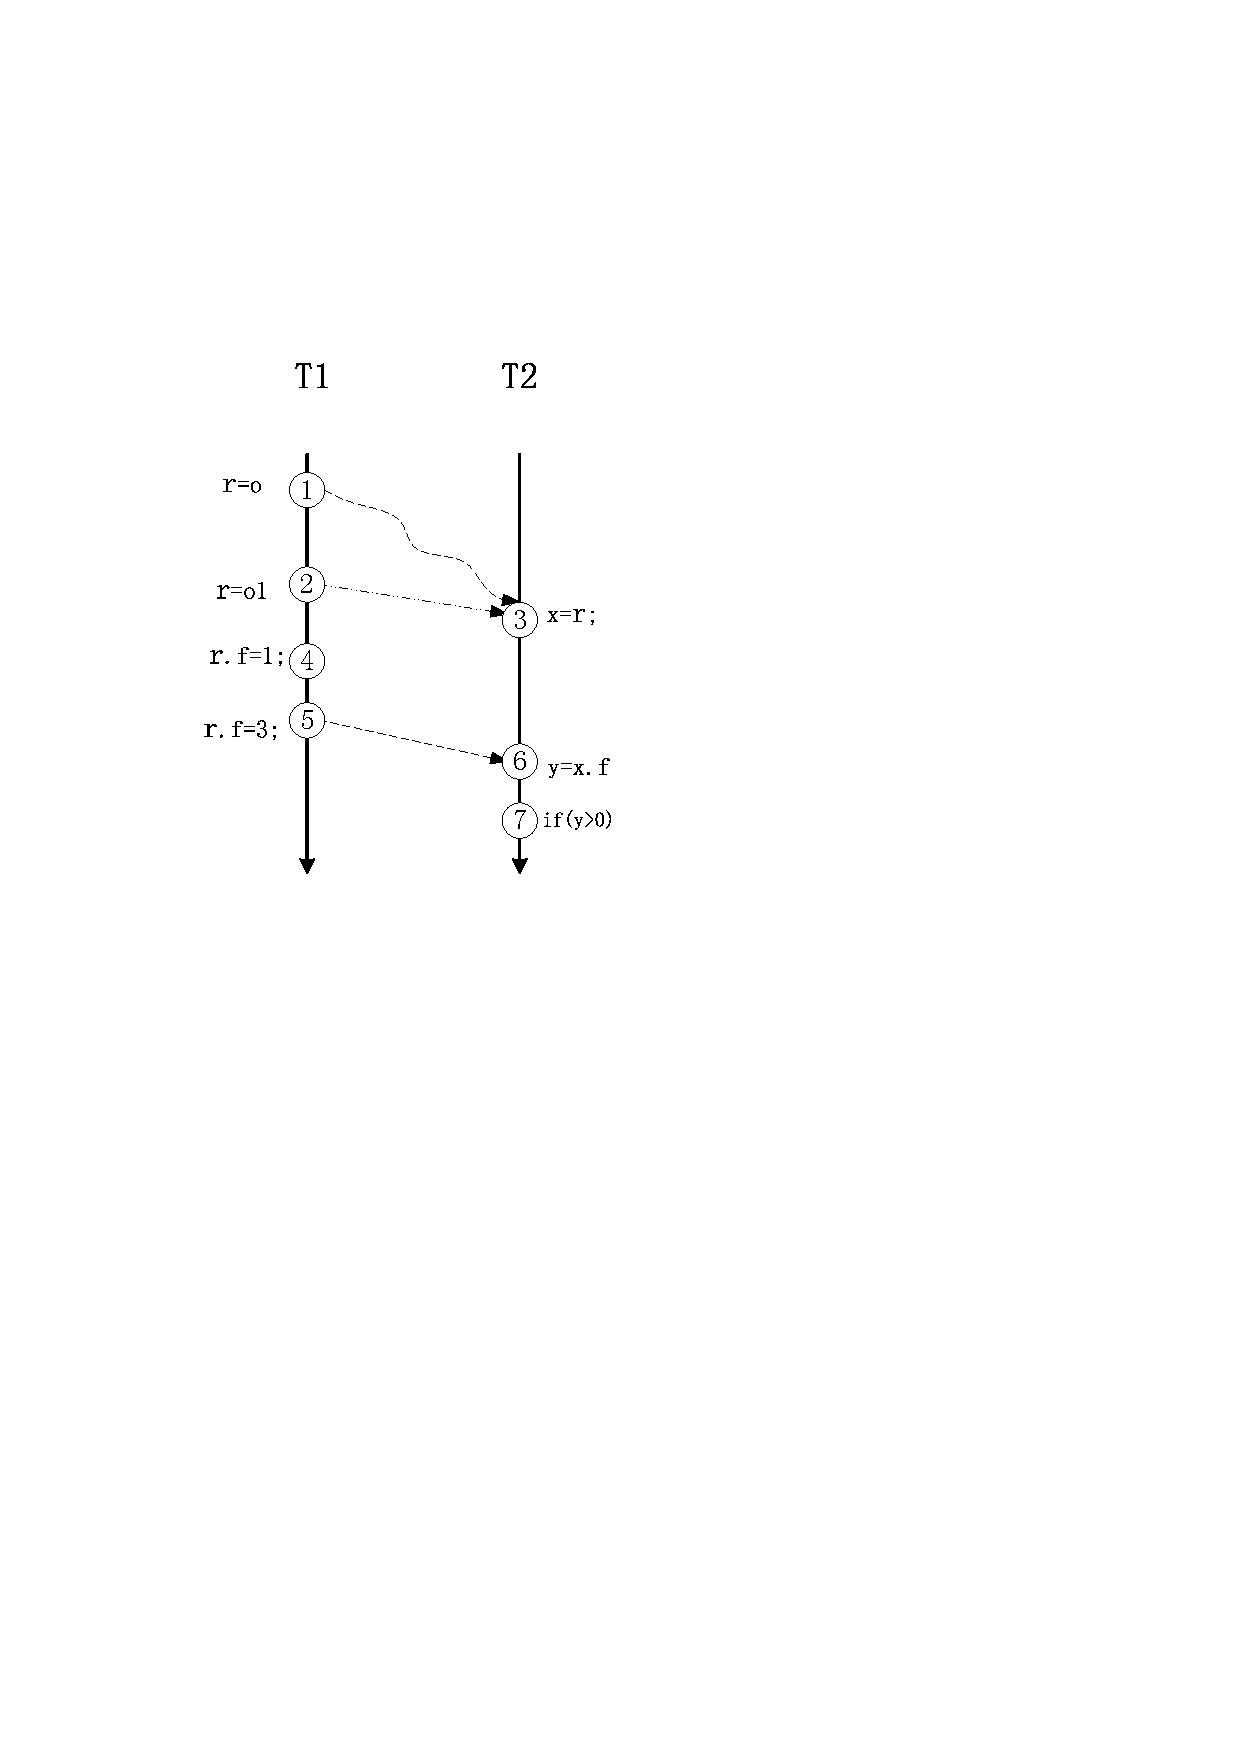
\includegraphics[scale=0.7]{figs/Visio-discuss.pdf}
\caption{Illustration of Detection Capability.}\label{fig:discuss}
\end{figure}




%
%In this section, we prove formally the soundness of \tool.
%
%Researchers~\cite{pldi14,maximal} propose two axioms, {\em prefix closedness} and {\em local determinism}, which we adapt to establish our feasibility guarantee. 
%Suppose $\mathcal{F}$ denotes the domain of feasible traces.
%
%
%Intuitively, Prefix closedness means that if a trace is feasible, then the trace is still feasible after we discard the events after a point. The underlying reason is that the events after a point cannot affect the events before it. More formally,
%
%\begin{myaxiom}[Prefix closedness]~\label{axiom:prefix}
%If $t_1$ $t_2$ $\in \mathcal{F}$, then $t_1 \in \mathcal{F}$. 
%\end{myaxiom}
%
%
%
%
%Intuitively, local determinism says that only the previous events of the same thread determine the existence of an event. For example, the existence of an event is only determined by the branch  thread-locally. However, the value read by an event may be affected by another thread because a shared read reads from the most recent write, which may come from a different thread. The value in other events, such as branch or write,  are locally determined too.
%More formally,
%
%
%
%
%
%\begin{myaxiom}[Local determinism]~\label{axiom:local}
%Assume $t_1e_1, t_2 \in \mathcal{F}$, and $t_1|thread(e_1)\approx t_2|thread(e_1)$, where $\approx$ denotes the two traces are equal if the data values in the read and write events are ignored, 
%Each event is determined by the previous events in the same thread. There are four cases:
%\begin{itemize}
%%TODO refine it.
%\item {\bf Branch\ }. If op($e_1$)=branch, and $e_1$ is in the form of $x<y$ (without loss of generality), then there exists values $v_x$, $v_y$ such that $t_2 e_1 [v_x/data_x, v_y/data_y] \in \mathcal{F}$. Here $e_1 [v_x/data_x]$ represents that we replace the value of $x$ from $data_x$ to $v_x$ in $e_1$.
%\item {\bf Read\ }. If op($e_1$)=read, and $e_2$ is a read event that is identical to $e_1$ except that it may read a different value, and $t_2 e_2$ is consistent, then $t_2 e_2 \in \mathcal{F}$.
%\item {\bf Write\ }. If op($e_1$)=write, and there is a value $v$ such that $t_2 e_1[v/data]\in \mathcal{F}$. 
%\item {\bf Others \ }. If op($e_1$) is of type different from above and $t_2 e_1$ is consistent, then $t_2 e_1 \in \mathcal{F}$.
%\end{itemize}
%
%Here, the consistency is defined as follows. 
%A trace is consistency iff it satisfies 
%\end{myaxiom}
%
%The local determinism resembles the version in ~\cite{pldi14,maximal}. A crucial difference is that, for the branch event, we do not require all reads thread locally before it to read the identical values as in the original trace $t_1 e_1$. Instead, we allow the previous reads to read different values as long as the branch event is evaluated to the same boolean value, which guarantees the existence of the following events. Such relaxation allows us to find more races, while still preserving the feasibility. 
%
%
%An important assumption of ours is, we assume all local accesses are recorded in the trace so that we can determine the boolean status of a branch event computationally. ~\cite{pldi14}, which assume the local accesses are not recorded and cannot determine the status computationally, have to enforce the reads before a branch to read the same values, leading to a weaker feasibility criterion. We believe our axiom captures the real-world scenario more faithfully.
%Another important assumption is for the read-write consistency, i.e., we assume the heap invariant, so that we know exactly which reads correspond to which writes in the predicted run.
%
%%\begin{myaxiom}
%%A set of traces $\mathcal{F}$ is feasible if it satisfies prefix closedness and local determinism axioms. 
%%\end{myaxiom}
%
%
%
%They are called axioms because they are the rules that the sequentially consistent system~\cite{maximal} should follow.
%We refer the readers to the detailed discussion~\cite{maximal, pldi14}.
%
%
%
%%TODO what is \Phi
%\begin{mytheorem}[Soundness]
%All traces in the closure $closure(t, \Phi)$, which includes $t$ and is closed under the derivations in Axioms~\ref{axiom:prefix}~\ref{axiom:local}, are feasible.
%\end{mytheorem}
%
%%$\theta_1(expr(e_1))=\theta_2(expr_{e_1})$, then $t_2 \e_1 \in \mathcal{F}$. Here $\theta_1, \theta_2$ represent the mappings between variables and values established prior to $e_1$ by the same thread $thread(e_1)$. $expr(e_1)$ is a helper function that returns the expression in the branch condition. 
%\begin{proof}
%We order the traces in $closure(t)$ as, $t_0=t, t_1, t_2, t_3, \dots t_n$. Clearly, $t_0$ is feasible. In the following, we prove by induction, i.e., assume $t_{n}$ is feasible, then $t_{n+1}$ which is derived from $S=\{t_0, \dots t_n\}$ should be feasible. There are several possible derivations.
%\begin{itemize}
%\item if $t_{n+1}$ is a prefix of $t'\in S$, then $t_{n+1}\in\mathcal{F}$ because of the prefix closedness. $t_{n+1}$ shares the same mappings as $t'$.
%\item if $t_{n+1}$ is derived from $t^1 e^1, t^2\in \mathcal{F}$, we have $t^1|thread(e^1)\approx t^2|thread(e^1)$.
%\begin{itemize}
%\item $op(e^1)=branch$ and $e^1= x<y$. Our solver computes a mapping $\theta^d$ of all relevant variables such that $\theta(x<y)=\theta^d(x<y)$, then 
%$t^2 e_1[\theta^d(x)/\theta(x),\theta^d(y)/\theta(y) ]  \in \mathcal{F}$. Note that the mapping computed by solver may be different from the mapping in the trace $t^1$.
%\item $op(e^1)=read$. Our solver ensures the read-write consistency, i.e., $t^2 e^2$ is consistent, then $t^2 e^2 \in \mathcal{F}$. Note that $e^2$ is the same as $e^1$ except that it may read a different value.
%\item $op(e^1)=write$. There exists a value $v$ such that $t^2 e^2[v/data]\in \mathcal{F}$, where $v$ is included in the mapping computed by the solver. 
%\item $op(e^1)$ is of other types. Our solver ensures the consistency, i.e., $t^2 e^1$ is consistent, then $t^2 e^2 \in \mathcal{F}$.
%\end{itemize}
%\end{itemize}
%\end{proof}
%
%
%
%\begin{mytheorem}[Maximality]
%$\forall t', s.t., t'|th\approx t|th for any thread th, if t'\notin closure(t,\Phi), t' is infeasible.$
%\end{mytheorem}
%
%\begin{proof}
%We sketch the proof. All traces that satisfy  $t'|th\approx t|th for any thread th$ 
%\end{proof}



%discussion.

%\section{Basics}~\label{sec:basic}


\subsection{Trace Terminology}
Our analysis starts with a trace $\tau$,  a sequence of events, $e_0, e_1, \dots, e_n$.  
There are three types of events in general.
\begin{itemize}
\item the shared access, which includes the read and write of the shared fields, e.g., $o.f$=$x$ and $x$=$o.f$.
\item the local access, which includes only the access of the local variable, e.g., $x=y+z$ or $v.f=x$ (where $v$ is a thread-local object).
\item the branch event, which evaluates the branch condition to true/false, e.g., $x>3$.
\item the synchronization event, which includes start/join, wait/notify, lock/unlock events, e.g., $lock(o)$
\end{itemize}



Each event $e_i \in \Sigma$ is a tuple, $<t, id, a, v, ins>$, where $t\in \mathcal{T}$ denotes the thread generating the event, $id\in \mathcal{ID}$ denotes the unique integer assigned to the event (event id), $a\mathcal{A}$ denotes the address of the object or field (if any) accessed in the event,  $v\in \mathcal{V}$ denotes the value of the definition (if any) in the event, and $ins\in \mathcal{INS}$ denotes the three-address instruction generating the event.  Specifically, the address of the object $o$ is denoted as $id(o)\in \mathcal{ID}$, which is a string value representing $o$ uniquely, the address of the static field $f$ is  $id(f)$ and the address of the instance object field $o.f$ is  $id(o)\_id(f)$. Besides, as the event is derived by instrumenting the three-address code and monitoring the instrumented execution. Therefore, each event can involve at most three operands. 


The trace supports its standard operations as follows.
\begin{itemize}
\item projection, e.g., $\tau|t$ returns~\footnote{This is the abbreviation for the complete form $\tau|Thread=t$ } the events from the thread $t$,  $\tau|a$ returns the event involving the address $a$.  
\item concatenation. $\tau'=\tau e$ represents the new trace by appending the event $e$ to $\tau$.
\item length $|\tau|$. 
\item selecting an element. $\tau[0]$ and $\tau[|\tau|-1]$ represents the first and last event in $\tau$.
\end{itemize}


%The modeling of synchronization event is standard and explained in existing work, so we focus on the rest two types of events in this paper.

In addition, we maintain auxiliary information as follows.
\begin{itemize}
\item $AT: \mathcal{A} \times \mathcal{T} \rightarrow \gamma$ is a function that returns a trace $\tau \in \gamma$ that contains only the accesses of the address $a \in \mathcal{A}$ by the thread $t\in \mathcal{T}$. Each trace $\tau$ in $\gamma$ is defined over the alphabet of events $\Sigma$, specifically, the trace is an empty trace $\epsilon$ or defined in this way:  $\forall 0\leq i\leq |\tau|,   \tau[i]\in \Sigma, and, \forall i\neq j, \tau[i]\neq \tau[j]$. 
\item $R: \mathcal{A} \rightarrow \gamma$ is a function that returns the read accesses of the address $a\in \mathcal{A}$.
\item $W: \mathcal{A} \rightarrow \gamma$ is a function that returns the write accesses of the address $a \in \mathcal{A}$.
\item $Sync: \mathcal{A} \rightarrow \gamma$ is a function that returns the synchronization events involving the address $a\in \mathcal{A}$. 
\end{itemize}


\subsection{Symbolic Trace}
To facilitate the symbolic analysis, we need to introduce symbols to represent the operands in each event. Symbols allow us to overcome the limitation of concrete dependences and allow us to explore more dependences symbolically. 

%shared access only, local access only




{\bf Local Variables\  }
Like other symbolic analysis~\cite{jeff,chao}, the symbolic trace should be in the SSA form, i.e., each variable is defined exactly once. This is because the constraint solver employed by the analysis requires each variable to hold only one value. Besides, we need to make sure each use still reads from the same definition thread-locally. 

The  simple procedure shows the construction of the symbolic trace for local variables defined or used. The symbols are constructed by combining the static instruction and the runtime event id. Lines 6-10 handles the local variable definition.  We build a symbolic variable $s$ for it by combining the variable name and the event id. The uniqueness of the event id guarantees that each symbolic variable is defined exactly once. In addition, we replace the variable to the symbolic variable in the instruction and record the replacement in $table$. Lines 3-5 updates the local variable used in each event so that it is replaced with the symbolic variable for the corresponding definition. Here, the corresponding definition and the use share the same variable name, therefore, we can easily find out the symbolic variable through looking up the $table$. 

The SSA form of the trace is different from the SSA form of the instruction as the SSA instruction can only distinguish definitions at different program points but cannot distinguish the definitions at different execution points that share the same program point.





\begin{algorithmic}[3]
\For {$e: \tau$}
 \State $ins\gets e.ins$ 
 \For {$ins.use:ins.uses$}
 \State $ins.use \gets table(ins.use)$
 \EndFor
  \If {$ins.def\neq null$}
    \State $ s\gets ins.def^{e.id}$
	\State $ table [ins.def \rightarrow s]$
	\State $ins.def\gets s$
 \EndIf
\EndFor
\end{algorithmic}


%TODO update the intro+moti, make sure the same style
\begin{figure}
\centering
\begin{tabular}{ll}
\multicolumn{2}{c}{{\tt {\bf x} = 0; {\bf y} = 0;}} \\
\hline
\multicolumn{1}{c}{$T_1$} & \multicolumn{1}{c}{$T_2$} \\
\hline
{\tt 1: s=0; } & \\
{\tt 2: for(i=1;i<3;i++)} & \\
{\tt 3: \ \ \ s+=i;} & \\
{\tt 4: {\bf y} = s;} & \\
{\tt 5: {\bf x} = 1;} & \\
{\tt 6: {\bf y} = 5;} & \\
& {\tt 7: if ({\bf y} > 2)} \\
& {\tt 8:~~print({\bf x}+1);} \\	
& {\color{Gray} {\tt 9: else}} \\
& {\color{Gray} {\tt 10:~~print({\bf x}+2);}}
\end{tabular}
\caption{Running Example (shared variables are in bold font). }
\label{fig:running2}
\end{figure}



{\bf Shared Accesses}   Besides, we introduce symbols to represent shared reads and shared writes which leave the inter-thread dependence between reads/writes undetermined. For each read (or write) of shared variable $x$, we introduce $R^{id}_x$ (or $W^{id}_x$) to denote it, where $id$ is the event id.
Consider the code in Figure~\ref{fig:running2}, which resembles the example in Figure~\ref{fig:running} except that it includes a for loop at lines 1-2.
The symbolic trace is produced in Figure~\ref{fig:t4running2}. For simplicity, we only show the symbolic variables, while omitting other information such as thread information.




%TODO distinguish T1 and T2 in the text. 
\begin{figure}
\centering
\begin{tabular}{l|l}
\hline
\multicolumn{1}{c}{$Trace$} & \multicolumn{1}{c}{$Symbolic\  Trace$} \\
\hline
{\tt 0: {\bf x}=0} &  {\tt 0: $W^0_x$=0}    \\
{\tt 1: {\bf y}=0} &   {\tt 1: $W^1_y$=0}   \\
{\tt 2: s=0} &  {\tt 2: $s^2$=0}   \\
{\tt 3: i=1} &     {\tt 3: $i^3$=1}   \\
{\tt 4: i<3} &    {\tt 4: $i^3$<3} \\
{\tt 5: s=s+i} & {\tt 5: $s^5$=$s^2$+$i^3$}   \\
{\tt 6: i=2} &       {\tt 6: $i^6$=2}  \\
{\tt 7: i<3} &      {\tt 7: $i^6$<3}  \\
{\tt 8: s=s+i} &  {\tt 8: $s^8$=$s^5$+$i^6$}  \\
{\tt 9: i=3} &     {\tt 9: $i^9$=3}  \\
{\tt 10: i<3} &    {\tt 10: $i^9$<3}  \\
{\tt 11: {\bf y} = s;} &  {\tt 11: $W^{11}_y$ = $s^8$;}  \\
{\tt 12: {\bf x} = 1;} &    {\tt 12: $W^{12}_x$ = 1;}   \\
{\tt 13: {\bf y} = 5;} &    {\tt 13: $W^{13}_y$ = 5;}  \\
{\tt 14: {\bf y} > 2}  &    {\tt 14: $R^{14}_y$ > 2} \\
{\tt 15: tmp={\bf x}+1;}  & {\tt 15: tmp=$R^{15}_x$+1;}   \\	
{\tt 16: print(tmp);} &  {\tt 16: print(tmp);}  \\
\end{tabular}
\caption{Trace}
\label{fig:t4running2}
\end{figure}



{\bf Method Calls\ } The key to supporting the method calls is to capture the value flow the actual argument to the formal argument, and the flow from the return statement to the LHS variable of the method call. To explicitly model the value flow, record two additional events for each method call.
Consider the example in Figure~\ref{fig:methcall},   we record the local access event $y1=y;$ for the argument value flow and record the  local access event $x=i2;$. Recording the additional events is achieved through instrumenting the call site and the callee method statically.  

The above simple strategy however hides the complexity of the virtual method calls. At a call site of a virtual method, the static instrumentation cannot know precisely which method would be called. Therefore, we do not know what formal argument the actual argument flows to. Consider the example in Figure~\ref{fig:methcall}, suppose another implementation of the virtual method exists (in the comments).  We do not know how to instrument the code statically, $y1=y$ or $y2=y$. 


To avoid the problem, we have to combine the runtime knowledge. 
Our strategy is as follows: rather than directly record direct value flow from actual argument to formal argument, we introduce an artificial variable during the static instrumentation. Then we  insert the instrumentation $record(ARG0=y;)$ at call site, and insert  $record(y1=ARG0)$ at the entry of the method $func$ declared in the first class, and insert $record(y2=ARG0);$ at the entry of the method $func$ declared in the second class. At runtime, depending on which $func$ method is invoked, we record either the event sequence $ARG0=y; y1=ARG0$ or the sequence $ARG0=y; y2=ARG0$, which precisely captures the value flow. We model the return value flow similarly. 

Note that although different methods use the same names for the artificial variable,  they are translated to different variables after we get the SSA form of symbolic trace. 

 

\begin{figure}
\centering
\begin{tabular}{ll}
{\tt  x=o.func(y) } &  \\ 
 {\tt  func(y1)\{ // class O1} &  \\
 {\tt  \ \      i=y1; } & \\
 {\tt  \ \      i2=2*i; } &  \\
 {\tt  \  \      return i2;} & \\ 
 {\tt           \}} & \\ 
 
  {\tt //  func(y2)\{ // class O2} &  \\
 {\tt  // \ \      j=y2; } & \\
 {\tt  // \ \      j2=3*j; } &  \\
 {\tt  // \  \      return j;} & \\ 
 {\tt  //         \}} & \\ 
\end{tabular}
\caption{Method Calls}
\label{fig:methcall}
\end{figure}





\subsection{Constraints}
The constraints 












\section{Time Window}~\label{sec:basic}

\section{Heap Invariant}~\label{sec:basic}

\section{Evaluation}~\label{sec:eval}
Our evaluation focuses on the effectiveness  and scalability.
To measure the effectiveness, we compare with the predictive analysis, 
{\sf RV}~\cite{pldi14}. We chose RV for two main reasons: (1) {\sf RV} is the 
only open source predictive analysis, (2) {\sf RV} represents the 
state-of-the-art, which is theoretically proven to have higher detection 
capability than other approaches. 

{\bf Prototype Implementation}  We use the Z3 SMT solver for constraint 
resolution \cite{MouraB08}. For static analysis, to discover unexecuted 
branches, we utilize the SOOT compiler framework \cite{Vallee-RaiCGHLS99}.

For scalability, as well as to constrain memory footprint, we have 
applied several engineering optimizations. In specific, (i) events are 
stored in a database rather than in an in-memory buffer; and (ii) the 
analysis is split into several segments, between which we restart 
the VM and resume the last snapshot, such that the different logs 
are fused together at the end. 

To improve the scalability in constraint solving, we again apply 
a splitting optimization. The full trace is split into $N$ equal-length 
subtraces or ``time windows'' (in our experiments, $N=1,000$). The values 
of local and shared variables are then passed at the end of a 
given window as the inputs to the next window. For lack of space, we 
omit the details, and instead refer the reader to 
Huang et al. \cite{pldi14}, who apply a similar optimization.


{\bf Evaluation Method} We conducted our experiments on a set of 16 
applications, which were also used to evaluate {\sf RV}. Specifically, 
the set includes large applications such as {\sf Jigsaw}, 
{\sf Xalan} and {\sf Lusearch}. To handle large applications that make 
use of reflection, we applied the {\sf Tamiflex} tool~\cite{tamiflex}, which 
replaces reflective calls with the concrete method invocations recorded 
in the observed run.
% for the purpose of effective static analysis.  
We omit the benchmark {\sf eclipse} because the current version 
of {\sf Tamiflex}  leads to abnormal execution after the instrumentation, 
which throws an exception when the main service is started. 
By applying \tool\  to the abnormal execution, we identify only 3 races, 
similarly to the report of RV~\cite{pldi14}.
In addition, the {\sf montecarlo} benchmark requires an external input 
that we downloaded from the internet and simplified. For the large 
applications, we utilized the most lightweight available configuration.


As the detection capability  depends on the observed run, for fair 
comparison we monitor the execution once by recording all necessary 
information required by both approaches, and then apply both techniques 
to the monitored run. Besides, our reported data for RV may be different 
from the original report for two reasons: (1) the different observed runs 
lead to different sets of races, (2) the original implementation of RV 
contains a bug in branch identification, which leads to  misses of 
many branches and  incorrect reduction of dependences during the analysis. 
We confirmed the bug with the author and fixed the bug in our 
experiments.\footnote{We have created an in-depth report on the bug, 
along with a witness test case. (See:  \url{https://sites.google.com/site/recipe3141/}.)}


Our experiments and measurements were all conducted on an x86 64 
Thinkpad W530 workstation with eight 2.30GHz Intel Core i7-3610QM, 
16GB of RAM and 6M cache. The workstation runs Ubuntu 12.04,
% of the Ubuntu Linux distribution, 
and has the Sun 64-Bit 1.6.0\_26 JVM installed.
%\footnote{We note that Sun JDK 1.7 does not support the transformation of dacapo applications with {\sf tamiflex}.}


%Specifically, we use two threads in the monitored run as two threads are sufficient to manifest most of races~\cite{shanlu}. 








\subsection{Effectiveness}
Table~\ref{tab:main} shows the main results of our analysis, which includes four sections: Trace (details about the trace), Races (detected races), Difference (comparison with RV) and Running time (the time taken by the analysis).


The Trace section includes the number of threads ($Th$), the number of 
shared reads ($Reads$) and shared writes ($Writes$), the subset of shared 
reads that read the base object references  ($Base$), where the  base object 
references are references used as the base/target in the following field 
reference or method invocation,  the number of branches ($Br$), the 
synchronization events ($Sync$) and the total number of events ($Total$), 
which includes local accesses in addition to the aforementioned events. 
Specifically, branch events are reported in the form $A/B$, where $A$ refers 
to the number of branches used by our analysis and $B$ refers to the number 
of branches used by RV. To ensure that the predicted run sees the same 
base object at each shared read/write, {\sf RV} inserts an artificial 
branch immediately in front of each shared access (and array accesses). 
We do not use such artificial branches.


We make a few interesting observations about the Trace section. 
The non-local events, i.e., all the events listed in Table~\ref{tab:main}, 
occupy around 30\% of the total trace in the first 7 benchmarks, 
but occupy less than 1\% of the trace in the rest of the benchmarks, 
which have relatively more complex logic. Reads of the shared base objects 
occupy a small portion ($\frac{1}{10}$-$\frac{1}{3}$) of the total 
shared reads. The rest of the shared reads read only primitive values 
or references not involved in field accesses (e.g., references involved 
in nullness checking). Besides, our analysis involves significantly less branch events as compared to the {\sf RV} approach. This difference plays an important role in the detection, which we will explain shortly.


The $Races$ section shows the number of races detected by {\sf Recipe-s}, 
i.e., {\sf Recipe} without exploring un-executed paths; {\sf Recipe}, i.e., the full-fledged version; and {\sf RV}. Comparison between {\sf Recipe-s} 
and {\sf Recipe} reveals that {\sf Recipe} finds $>$100 more races, 
which demonstrates the strength of exploring  un-executed paths. 
Intuitively,  {\sf Recipe-s} predicts based on a single trace, while 
{\sf Recipe} predicts based on multiple traces containing different 
execution paths. We also compare between {\sf Recipe} and {\sf RV} version, 
as shown in the $Difference$ section, where $Diff$ shows the races found 
by {\sf Recipe} but missed by {\sf RV} while $Diff'$ shows the races 
found by {\sf RV} but not {\sf Recipe}.

First of all, {\sf Recipe} finds $>$150 more races than {\sf RV}. There 
are several reasons for that: (1) {\sf Recipe} can reason about the 
accesses in the un-executed paths, while {\sf RV} and {\sf Recipe-s} can 
only reason about the accesses in the executed paths. (2) {\sf Recipe} 
or {\sf Recipe-s} relax the scheduling even if it 
%breaks the inter-thread read/write dependence structure 
changes variable values in the observed run. {\sf Recipe} allows the 
majority of the shared reads, i.e., the reads of primitive values, 
to freely read a different value from a different write 
as long as the value leads to the same branch decisions. {\sf RV}, however, 
requires them to read the same values as in the observed run. (3) An 
critical optimization proposed by {\sf RV} is to preserve dependences 
only for the reads before the preceding branches of the racy events, 
rather than all the reads. However, this optimization is underplayed 
by the fact that {\sf RV} introduces huge amount of artificial 
branches, i.e., one before each shared field access, which ensures 
the use of the same base objects.
We get rid of such artificial branches and instead, rely on the small 
amount of base read events to ensure the use of the same base 
objects (Section~\ref{sec:relax1} and Section~\ref{sec:relax2}). Our strategy reduces the number of branches 
greatly and amplifies the effectiveness of the optimization. We also 
carried out case studies (Section~\ref{sec:cases}) to better illustrate the scenarios.

 

Another interesting observation is that although {\sf Recipe} should 
produce all races found by {\sf RV} in theory, {\sf Recipe} may miss 
races found by {\sf RV} in practice (Column $Diff'$), i.e., {\sf Recipe} 
is not strictly more effective than {\sf RV} in practice. The reason  is 
the limitations of the underlying constraint solver: (1) the solver cannot 
compute constraints with very complex arithmatic operations, and (2) the 
solver does not support some program constants such as the scientific 
notation $3E-10$. In our empirical evaluation, we encounted only one 
benchmark, account, where these issues manifested.

The last section, Running time, compares the analysis time for both 
approaches. We find our approach is significantly slower than {\sf RV}, 
e.g., {\sf RV} often finishes within 200 seconds, while our approach may 
take more than 1 hour. This is because {\sf Recipe} has a larger search 
space and needs to reason about the computation among variables inside 
the local access events, while {\sf RV} needs to only reason about 
the order relations among the events.


 











%TODO Reorder the columns: RV ReceipeS Recipe


\begin{table*}[htbp]
\caption{Relaxed Analysis}
\begin{flushleft}
\begin{tabular}{|l|r|r|r|r|l|r|r|r|r|r|r|r|r|r|}
\hline
 & \multicolumn{ 7}{c|}{Trace} & \multicolumn{ 3}{c|}{Races} & \multicolumn{ 2}{c|}{Difference} & \multicolumn{ 2}{c|}{Running time (sec)} \\ \hline
Benchmarks & \multicolumn{1}{l|}{Th} & \multicolumn{1}{l|}{Reads} & \multicolumn{1}{l|}{Writes} & \multicolumn{1}{l|}{Base} & Br & \multicolumn{1}{l|}{sync} & \multicolumn{1}{l|}{Total} & \multicolumn{1}{l|}{Recipe-s} & \multicolumn{1}{l|}{Recipe} & \multicolumn{1}{l|}{RV} & \multicolumn{1}{l|}{Diff} & \multicolumn{1}{l|}{Diff'} & \multicolumn{1}{l|}{Recipe} & \multicolumn{1}{l|}{RV} \\ \hline
critical & 3 & 13 & 7 & 5 & 2/13 & 6 & 78 & 8 & 8 & 8 & \multicolumn{1}{c|}{0} & 0 & 8 & \multicolumn{1}{c|}{2} \\ \hline
airline & 11 & 45 & 15 & 4 & 32/82 & 30 & 317 & 9 & 9 & 9 & 0 & 0 & 490 & 4 \\ \hline
account & 3 & 46 & 21 & 10 & 3/47 & 6 & 227 & 2 & 5 & 5 & 3 & 3 & 41 & 4 \\ \hline
pingpong & 4 & 7 & 7 & 3 & 0/15 & 6 & 111 & 1 & 1 & 1 & 0 & 0 & 19 & 1 \\ \hline
bbuffer & 4 & 640 & 118 & 10 & 634/1.1K & 217 & 3.3K & 13 & 25 & 9 & 21 & 5 & 62 & 5 \\ \hline
bubblesort & 26 & 1.3k & 966 & 121 & 155/2.8K & 322 & 8.4K & 7 & 7 & 7 & 0 & 0 & 3295 & 3 \\ \hline
bufwriter & 5 & 165 & 52 & 75 & 16/130 & 44 & 525 & 4 & 10 & 2 & 8 & 0 & 63 & 9 \\ \hline
mergesort & 5 & 38 & 33 & 5 & 15/472 & 28 & 1.7K & 3 & 10 & 3 & 10 & 0 & 37 & 5 \\ \hline
raytracer & 2 & 31 & 5 & 12 & 314/8,2K & 676 & 94.5K & 4 & 6 & 4 & 2 & 0 & 47 & 2 \\ \hline
montecarlo & 2 & 5 & 86 & 2 & 1.9K/38.2K & 21.1K & 1.9M & 1 & 4 & 1 & 3 & 0 & 1 & 17 \\ \hline
moldyn & 2 & 605 & 61 & 104 & 19.6K/52.6K & 62 & 203.4K & 6 & 14 & 2 & 12 & 0 & 2842 & 1 \\ \hline
ftpserver & 28 & 684 & 299 & 71 & 4.4K/233.3K & 78.2K & 3.9M & 99 & 152 & 57 & 108 & 13 & 811 & 153 \\ \hline
jigsaw & 12 & 525 & 702 & 211 & 63.2K/467.9K & 86.7K & 5.5M & 17 & 23 & 8 & 15 & 0 & 33 & 7 \\ \hline
sunflow & 9 & \multicolumn{1}{l|}{2.1K} & \multicolumn{1}{l|}{1.3K} & 473 & 201.3K/827.0K & 50K & \multicolumn{1}{l|}{7.1M} & 38 & 78 & 20 & 69 & 11 & 4520 & 22 \\ \hline
xalan & 9 & \multicolumn{1}{l|}{1.4K} & \multicolumn{1}{l|}{0.9K} & 209 & 15.7K/103.2K & \multicolumn{1}{l|}{190.1K} & \multicolumn{1}{l|}{6.6M} & 2 & 6 & 2 & 4 & 0 & 5317 & 10 \\ \hline
lusearch & 10 & \multicolumn{1}{l|}{2.3K} & \multicolumn{1}{l|}{0.5K} & 715 & 22.2K/164K & \multicolumn{1}{l|}{93.2K} & \multicolumn{1}{l|}{9.1M} & 27 & 49 & 14 & 38 & 5 & 5430 & 8 \\ \hline
\end{tabular}
\end{flushleft}
\label{tab:main}
\end{table*}









  



\subsection{Case studies}~\label{sec:cases}
We manually inspected the reported races over small applications to gain better understanding about our approach. 

{\bf Relaxing Values\ } Figure~\ref{fig:relax1} demonstrates the relaxation of inter-thread dependence enabled by our approach. 
The code is from the benchmark {\sf bbuffer}, where the line numbers are
marked. Huang et al.~\cite{pldi14} detect the race between lines 291 and 400, 
but fail to detect the race between lines 294 and 400. The reason is 
that in the observed run, the execution follows the order 400, 291 and 294. 
For the event at line 294, its preceding branch at line 291 reads 
from line 400. Therefore, Huang et al.~\cite{pldi14}
require the predicted run to preserve the dependence between line 291 and 
line 400, so that line 291 reads exactly the same value and the branching 
expression evaluates to the same truth value. The dependence enforces 
the order constraint, $400 \rightarrow 291$, which further enforces 
the order $400\rightarrow 291 \rightarrow 294$.    Our approach does not 
require the existence of such dependence. Specifically, we allow line 
291 to happen before line 400 in the predicted run as long as the value 
read by it leads to the same branch decision, which is true in this case.  
As a result, there is no order constraint between line 294 and 
line 400, and the two form a race. We were able to replay this race  
easily using the eclipse IDE breakpoints. 


 

\begin{figure}[htp]
\centering
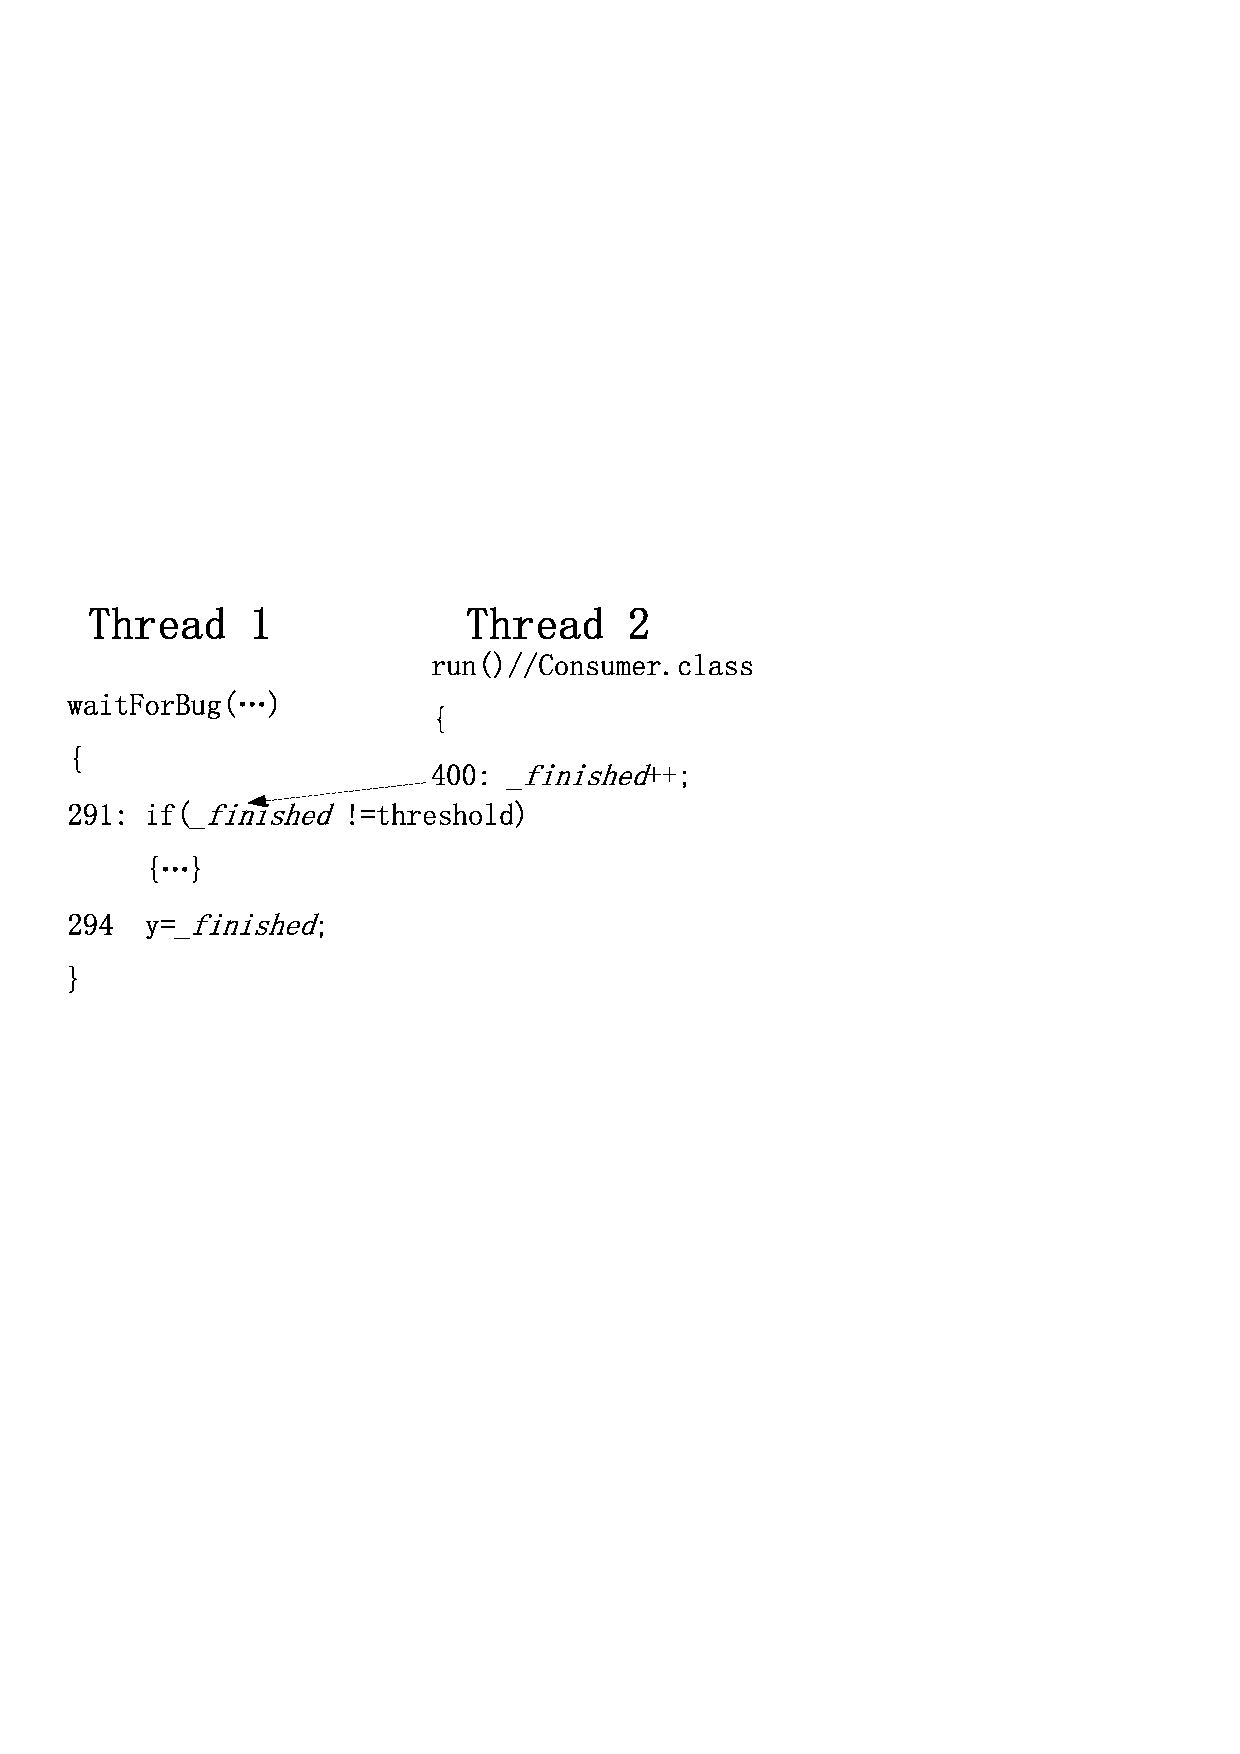
\includegraphics[scale=0.45]{figs/Visio-bbuffer.pdf}
\caption{Relaxation of Inter-thread dependence}\label{fig:relax1}
\end{figure}

{\bf Relaxing the Paths\ } Figure~\ref{fig:relax2} demonstrates how our 
approach relaxes the scheduling to account for  unexecuted paths in 
{\tt mergesort}. 
All threads invoke the method {\sf Sorting}, which recursively starts 
two child threads if there are two more available entries in the 
thread pool (lines 8-11), or starts one child thread if there is only 
one available entry (lines 4-5).  The availability is computed through 
the static method {\sf available} with the constant {\tt total}, which is equal to 5. The shared variable {\tt alive} denotes the used entries.

 
Initially there is one sorting thread. After it starts Thread 1 and 
Thread 2, there are three threads alive and only two more 
entries are available. Suppose that in the observed run Thread 2 
consumes both thread entries and starts the child Thread 3 
and Thread 4 (not shown), updating {\tt alive} to 5. Then Thread 1 
cannot execute the branch at lines 4-5. Huang et al.~\cite{pldi14} require the predicted run to preserve the dependence denoted by the dotted line since this dependence affects the branch condition at line 2. As a result, the predicted run follows the same branch decision and cannot reason about the code at lines 4-5. Our analysis does not suffer from this limitation. Instead, it allows the predicted run to reason about the un-explored code. Specifically, it does not need to preserve the dependence from line 11 to line 1, and it allows line 1 (Thread 1) to read from line 9 (Thread 2). As a result, the branch condition guarding the unexplored branch is evaluated to be true, enabling the unexplored path in the constraint solver. Finally, the solver identifies the race between line 5 (Thread 1) and line 1 (Thread 3). Note that the two lines are synchronized on different locks~\footnote{We abbreviate the {\tt synchronized} keyword as {\tt sync}.
}. 

 


\begin{figure}[htp]
\centering
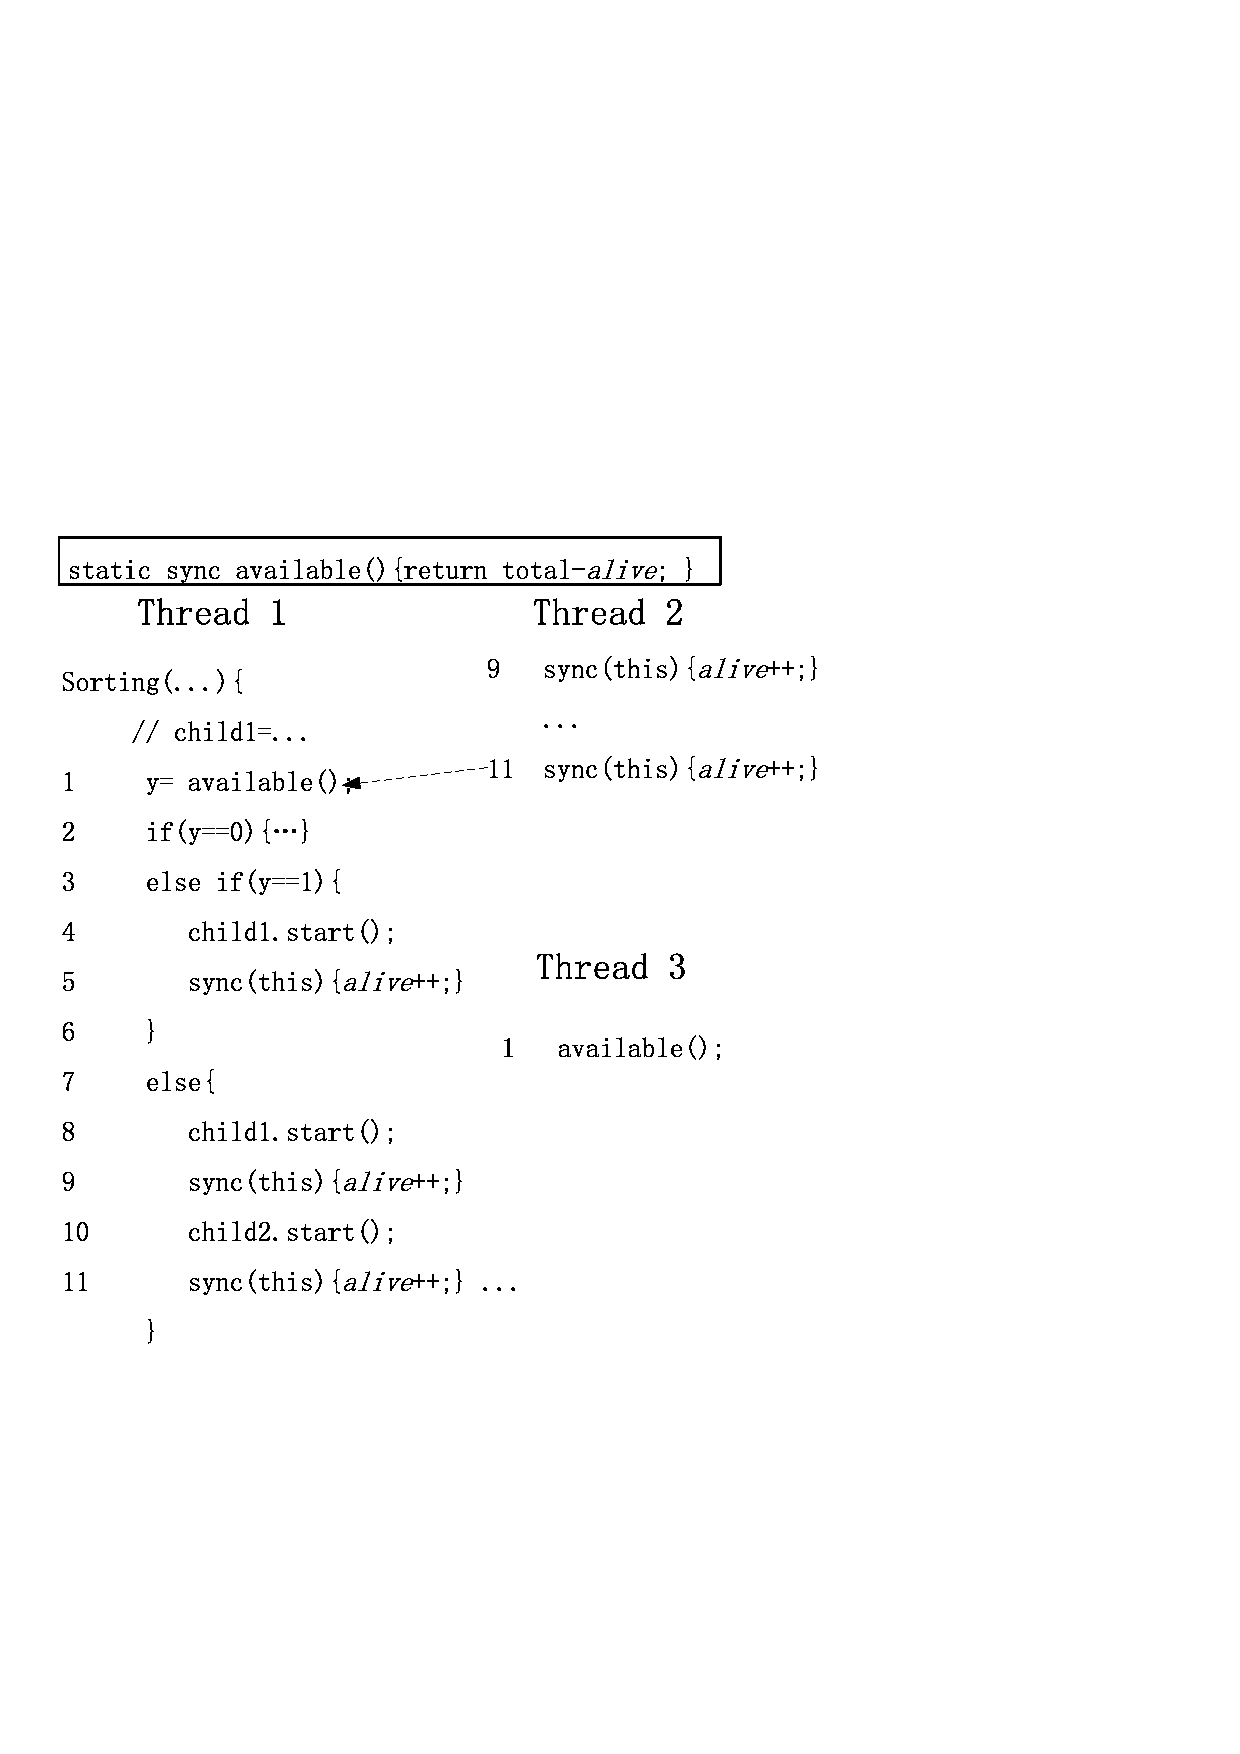
\includegraphics[scale=0.45]{figs/Visio-msort.pdf}
\caption{Relaxation of Paths}\label{fig:relax2}
\end{figure}


\section{Threats to Validity}
A Java method can consist of up to 65535 bytecode instructions. Therefore,
 we count the number of bytecode instructions inside each method. If the 
resulting number exceeds 65525, we avoid instrumenting the method. 
The consequence is that we will potentially miss races inside a method for 
which we skipped instrumentation. In this case, we specify the variables 
read from the method to be equal to their concrete values in the constraints. 
The constraint solver can proceed safely without being affected by 
such methods.

\tool lacks support for certain operators. In our current 
implementation, we do not support bit operations such as $\&$ and $<<$, which accounts for most of our misses.




\section{Related Work}

%In this section, we survey related research on race detection with special emphasis on predictive trace analysis (PTA).

\subsection{Race Detection Techniques: Broad Survey} 

Initial attempts to address the challenge of race detection focused on 
built-in synchronization primitives \cite{eraser,SasturkarAWS05,vonPraun:2001,
Choi:2002}. These include locks as well as the wait/notify and start/join 
primitives. Notable among these efforts is the \emph{lockset} analysis, 
which considers only locks \cite{eraser}. Because the derived constraints 
are partial, permitting certain infeasible event reorderings, lockset 
analysis cannot guarantee soundness \cite{Naik:2006}. 

A different tradeoff is struck by the \emph{happens-before (HB)} 
approach \cite{Christiaens,Dinning:1990,Mellor-Crummey:1991}, which is 
founded on Lamport's HB relation \cite{Lamport}. In HB analysis, all 
synchronization primitives are accounted for, though reordering constraints 
are overly conservative. 
%As an example, HB inhibits reordering of two synchronized 
%blocks governed by the same lock. 

%PTA is an instance  of the HB approach, whose starting point is a concrete execution trace.

Recently there have been successful attempts to relax HB constraints, including
%Among these are 
the hybrid analysis \cite{hybrid}, which permits both orderings of 
lock-synchronized blocks, and the \emph{Universal Causal Graph (UCG)} 
representation~\cite{ucg}, which also enables both orderings but only 
if these are consistent with wait/notify- and start/join-induced constraints.

\subsection{Predictive Trace Analysis (PTA)}

Given a concurrent execution trace $t$, PTA derives new traces to witness 
the data races. PTA is founded on the notion of sound causality, as it 
considers feasible reorderings of the input trace that prove a candidate 
data race as such. 

Wang et al.~\cite{chao} pioneere the symbolic predictive analysis, 
which our approach also belongs to. However, the approach lacks support 
of heap encoding, therefore, cannot be applied to real-world applications. 
The first PTA that applies to real-world applications is proposed by 
Smagardakis et al. \cite{yannis}. In their original work, both synchronization 
constraints and inter-thread dependencies are preserved, where inter-thread 
dependencies are respected by only allowing reorderings that leave the 
dependence structure exhibited by the original trace intact. This ensures 
that the values of shared memory locations remain the same, which secures 
the soundness argument.

Said et al. \cite{Said:2011} and Huang et al. \cite{HuangMR14} proposed
PTAs that are also sound. Said et al. perform symbolic analysis of the 
input trace, and then utilize an SMT solver to search for schedules that 
establish the presence of data races. Soundness is guaranteed by their 
ability to precisely encode the semantics of sequential consistency. 
Inspired by Said et al., Huang et al. present an improvement, whereby 
control-flow information is encoded into the constraint system so as 
to relax flow dependencies as long as control dependencies are 
preserved. ExceptionNULL \cite{Farzan:2012} is another example of 
sound PTA. Its goal is to detect null dereferences rather than data races. 

\tool\ is similar to Said et al. and Huang et al. in that it also makes 
use of an SMT solver based on symbolic encoding of the input 
trace. Still, the two sound relaxations that \tool\ features, which 
enable (i) value- rather than dependence-based reasoning about data 
flow and (ii) consideration of unexplored branches, are strictly beyond
the scope of both techniques. In Section \ref{sec:eval}, we demonstrate 
via direct comparison with Huang et al. the substantial improvement 
in coverage thanks to these relaxation methods.
%, which we prove to handle 
%in a sound manner.

\subsection{Maximality Claim}
Serbanuta et al. \cite{maximal} and Huang et al.~\cite{HuangMR14} both 
claim maximality of the detection capability, but under different assumptions. 
Assuming branch events are not modeled in the trace, \cite{maximal} guarantees maximality. Given few 
information in the trace, it conservatively requires the shared read to 
obtain the same value in the predicted run to ensure soundness. However, if 
branch events are modeled, the technique does not guarantee maximality.  
Assuming the branch events are modeled but local assignments are not recorded, 
\cite{HuangMR14} guarantees maximality. 
Compared to \cite{maximal}, it allows some events to read different 
values if they do not affect the following branch decisions. However, 
it requires the events that affect the branch decisions to read exactly 
the same values. In practice, these assumptions are too restrictive  
because local assignments can be easily collected in practice.
%the testers often have full access to the source/bytecode and 
%can collect local assignments freely.  

Assuming local assignments are available in the trace, both techniques 
cannot guarantee maximality. As illustrated in our example and discussed 
in Section~\ref{sec:guarantee}, our analysis allows higher detection capability
%, i.e., we allow the events to read different values even they flow into the branch events; we allow the exploration of un-executed paths, both of which are not allowed by the above techniques.
 




% An example of a floating figure using the graphicx package.
% Note that \label must occur AFTER (or within) \caption.
% For figures, \caption should occur after the \includegraphics.
% Note that IEEEtran v1.7 and later has special internal code that
% is designed to preserve the operation of \label within \caption
% even when the captionsoff option is in effect. However, because
% of issues like this, it may be the safest practice to put all your
% \label just after \caption rather than within \caption{}.
%
% Reminder: the "draftcls" or "draftclsnofoot", not "draft", class
% option should be used if it is desired that the figures are to be
% displayed while in draft mode.
%
%\begin{figure}[!t]
%\centering
%\includegraphics[width=2.5in]{myfigure}
% where an .eps filename suffix will be assumed under latex,
% and a .pdf suffix will be assumed for pdflatex; or what has been declared
% via \DeclareGraphicsExtensions.
%\caption{Simulation Results}
%\label{fig_sim}
%\end{figure}

% Note that IEEE typically puts floats only at the top, even when this
% results in a large percentage of a column being occupied by floats.


% An example of a double column floating figure using two subfigures.
% (The subfig.sty package must be loaded for this to work.)
% The subfigure \label commands are set within each subfloat command, the
% \label for the overall figure must come after \caption.
% \hfil must be used as a separator to get equal spacing.
% The subfigure.sty package works much the same way, except \subfigure is
% used instead of \subfloat.
%
%\begin{figure*}[!t]
%\centerline{\subfloat[Case I]\includegraphics[width=2.5in]{subfigcase1}%
%\label{fig_first_case}}
%\hfil
%\subfloat[Case II]{\includegraphics[width=2.5in]{subfigcase2}%
%\label{fig_second_case}}}
%\caption{Simulation results}
%\label{fig_sim}
%\end{figure*}
%
% Note that often IEEE papers with subfigures do not employ subfigure
% captions (using the optional argument to \subfloat), but instead will
% reference/describe all of them (a), (b), etc., within the main caption.


% An example of a floating table. Note that, for IEEE style tables, the
% \caption command should come BEFORE the table. Table text will default to
% \footnotesize as IEEE normally uses this smaller font for tables.
% The \label must come after \caption as always.
%
%\begin{table}[!t]
%% increase table row spacing, adjust to taste
%\renewcommand{\arraystretch}{1.3}
% if using array.sty, it might be a good idea to tweak the value of
% \extrarowheight as needed to properly center the text within the cells
%\caption{An Example of a Table}
%\label{table_example}
%\centering
%% Some packages, such as MDW tools, offer better commands for making tables
%% than the plain LaTeX2e tabular which is used here.
%\begin{tabular}{|c||c|}
%\hline
%One & Two\\
%\hline
%Three & Four\\
%\hline
%\end{tabular}
%\end{table}


% Note that IEEE does not put floats in the very first column - or typically
% anywhere on the first page for that matter. Also, in-text middle ("here")
% positioning is not used. Most IEEE journals/conferences use top floats
% exclusively. Note that, LaTeX2e, unlike IEEE journals/conferences, places
% footnotes above bottom floats. This can be corrected via the \fnbelowfloat
% command of the stfloats package.


\section{Conclusion}
%\section{Conclusion and Future Work}
We develop \sysname, a relaxed predictive analysis technique. It has two
critical relaxations on existing predictive analysis that substantially
enlarge analysis coverage. The first relaxation allows variables to 
take different values as long as doing so does not affect trace feasiblity;
the second relaxation allows exploring neighboring unexecuted paths as long
as doing so does not affect the soundness guarantee. Our results show that
\sysname\  is able to detect 2.5X as many races as compared to the state-of-the-art,
without any false positives.

%In this paper, we investigated the problem of sound data-race detection (i.e., without false alarms) via predictive analysis
%The idea underlying predictive analysis is to start from a concrete --- and thus feasible --- execution trace, and apply transformations to the trace that are guaranteed to preserve feasibility while enjoying the concrete information encoded into the trace (such as concrete values, method resolutions, etc). 
%
%Two main limitations of the state of the art in predictive race detection, which we address as the main contributions of this paper, are (i) inability to guarantee feasibility while relaxing flow dependencies and (ii) inability to explore execution paths beyond the one in the input trace. 
%We have implemented \sysname, which we prove formally to be able to lift both of these limitations while guaranteeing soundness. We further demonstrate experimentally that thanks to its ability to explore more trace transformations, \sysname\ is able to detect x2.5 more races compared to the state of the art, and that both of the relaxation techniques \sysname\ features are important in achieving this result.

%An interesting topic for future research is how to combine our approach 
%with a lightweight approach with soundness guarantees like {\sf RV}. 
%One option is staged analysis, wherein {\sf RV} is run first. \tool\ is then left to run only on racy pairs not confirmed by {\sf RV}.
%In this way, we can also tackle misses due to practical limitations of the constraint solver.




% conference papers do not normally have an appendix


% use section* for acknowledgement
\section*{Acknowledgment}


The authors would like to thank...





% trigger a \newpage just before the given reference
% number - used to balance the columns on the last page
% adjust value as needed - may need to be readjusted if
% the document is modified later
%\IEEEtriggeratref{8}
% The "triggered" command can be changed if desired:
%\IEEEtriggercmd{\enlargethispage{-5in}}

% references section

% can use a bibliography generated by BibTeX as a .bbl file
% BibTeX documentation can be easily obtained at:
% http://www.ctan.org/tex-archive/biblio/bibtex/contrib/doc/
% The IEEEtran BibTeX style support page is at:
% http://www.michaelshell.org/tex/ieeetran/bibtex/
%\bibliographystyle{IEEEtran}
% argument is your BibTeX string definitions and bibliography database(s)
%\bibliography{IEEEabrv,../bib/paper}
%
% <OR> manually copy in the resultant .bbl file
% set second argument of \begin to the number of references
% (used to reserve space for the reference number labels box)
%\begin{thebibliography}{1}
%\bibitem{IEEEhowto:kopka}
%H.~Kopka and P.~W. Daly, \emph{A Guide to \LaTeX}, 3rd~ed.\hskip 1em plus
%  0.5em minus 0.4em\relax Harlow, England: Addison-Wesley, 1999.
%\end{thebibliography}

\bibliographystyle{abbrv}
\bibliography{paper}  % sigproc.bib is the name of the Bibliography in this case


% that's all folks
\end{document}


